\documentclass{article}
\usepackage{ctex}
\usepackage{graphics}
\usepackage{svg}
\usepackage{geometry}
\usepackage{subcaption}
\usepackage{minted}
\usepackage{pdfpages}
\geometry{a4paper, scale=0.75}
\begin{document}
    \section{实验目的}
    通过迭代式开发,深入掌握C语言的文件、链表、结构体、动态内存管理等技术,
    开发实现一个计费管理软件。同时在开发中使用了C++,Qt编写图形页面,对面向对象,GUI,有了初步认识。
    \section{系统功能与描述}
    \subsection{总体结构}
    \begin{figure}[hbt]
        \centering
        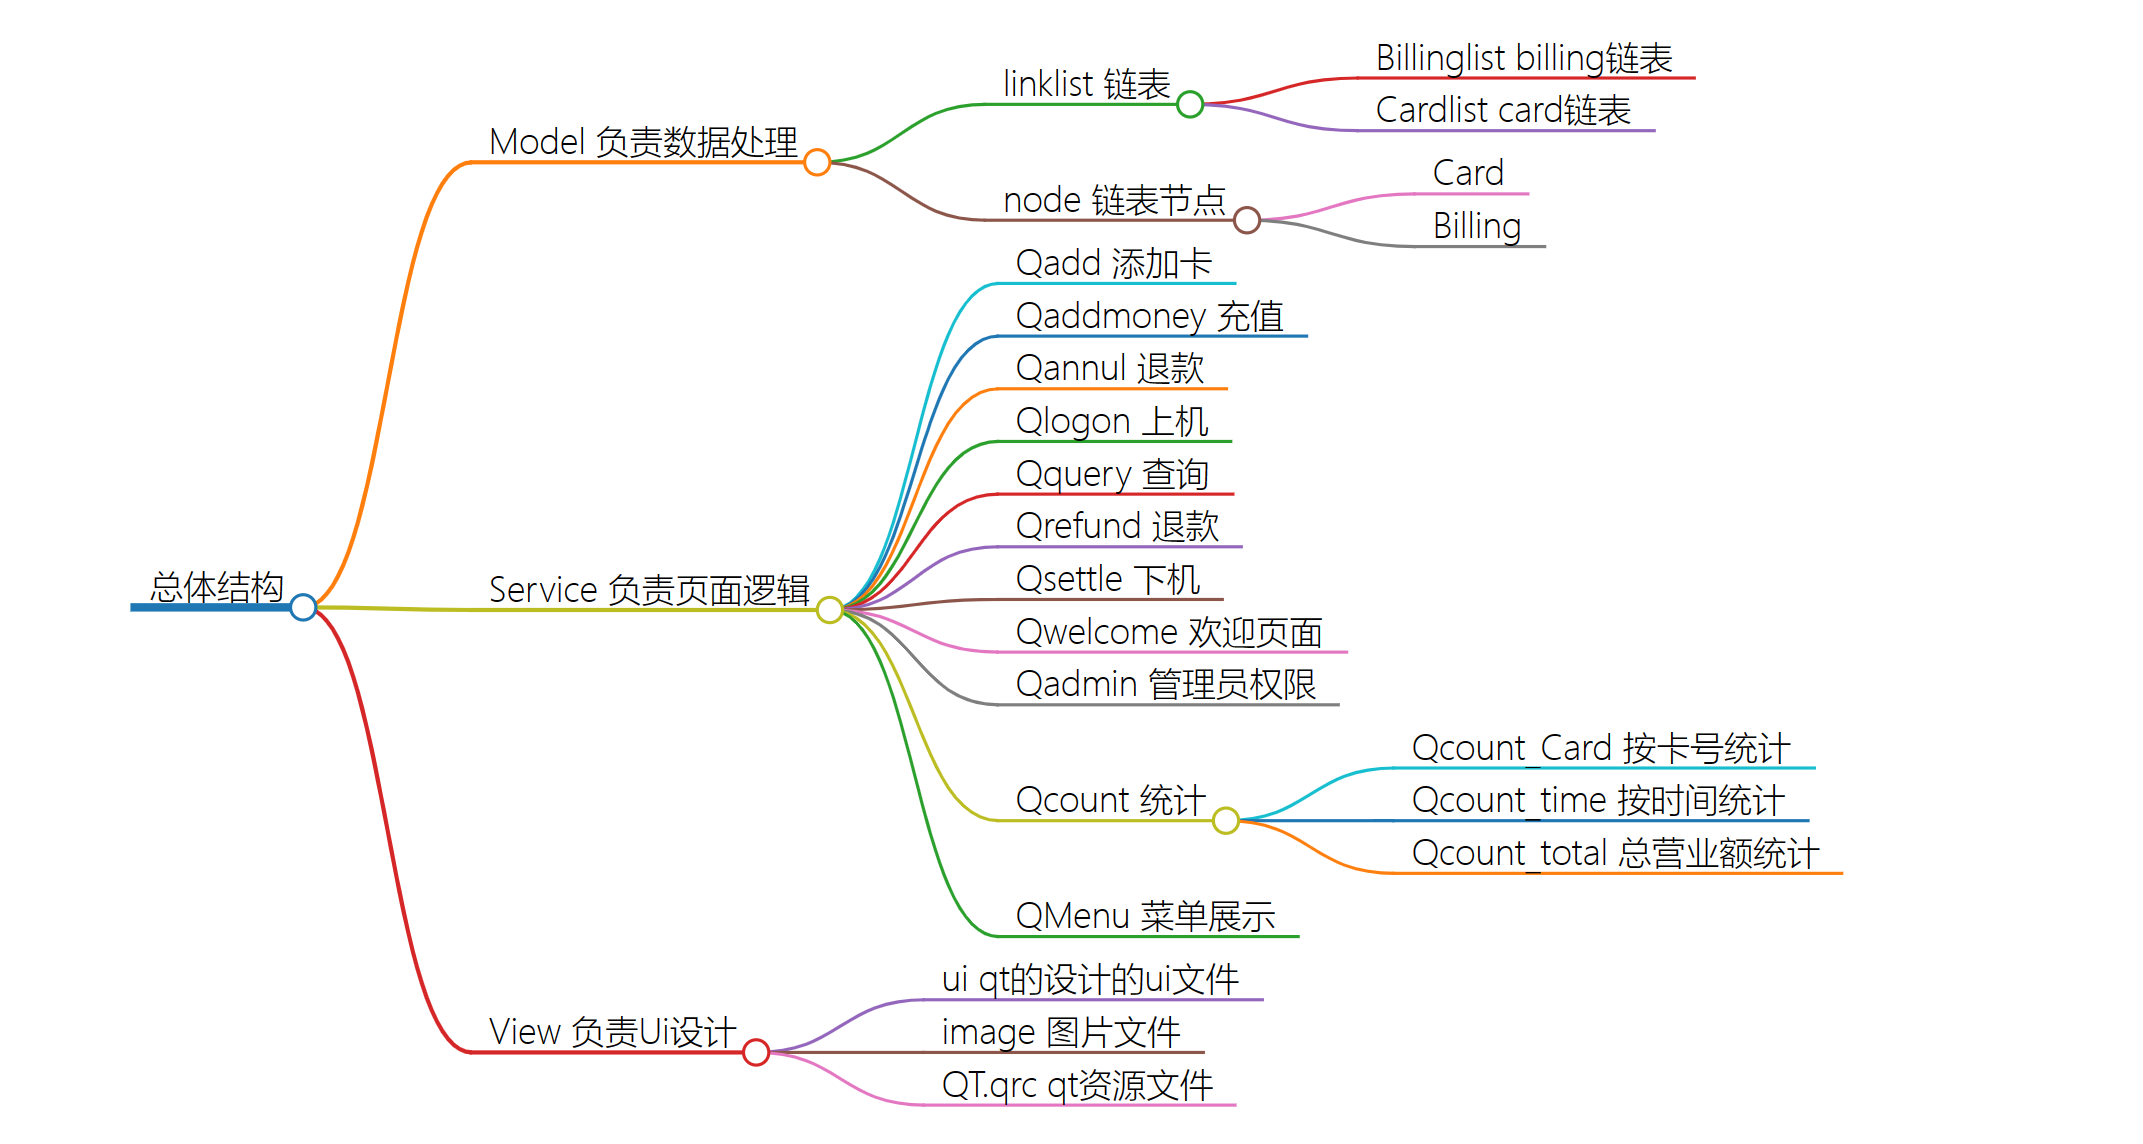
\includegraphics[scale=0.5]{figure/struct.png}
        \caption{总体结构}
        \label{struct}
    \end{figure}
    如图\ref{struct}为该程序总体结构,分为Model,Service,View三层结构
    \subsection{基础功能介绍}
    \subsubsection{菜单}
        \newpage
        \begin{figure}[h]
            \centering
            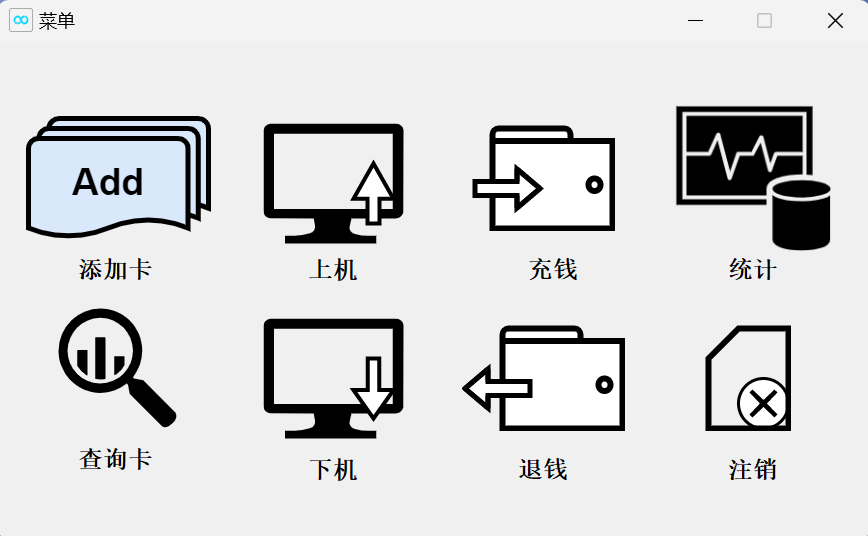
\includegraphics[scale=0.8]{figure/menu.png}
            \caption{主菜单}
            \label{main_menu}
        \end{figure}
        程序运行后进入主页面,如图\ref{main_menu},用户可以根据自己需求点击相应按钮进入该功能的页面。
        目前提供的功能有添加卡,上机,下机,查询卡,充钱,退钱,统计,注销六个功能
    \subsubsection{添加卡}
    \begin{minipage}[h]{0.5\linewidth}
        \paragraph{功能介绍}
        如右图,用户根据指引输入卡号,
        密码,开卡金额后点击OK就可以添加卡.
        \vfill
        \paragraph{返回结果}
        \begin{enumerate}
            \item 成功,则返回\ref{add_success}
            \item 卡号与已申请卡号重复,则返回\ref{id_repeat}
            \item 输入开卡金额非正,则返回\ref{add_less_zero}
            \item 输入卡号或密码过长,则返回\ref{too_long}。
        \end{enumerate}
    \end{minipage}
    \begin{minipage}[h]{0.5\linewidth}
        \centering
        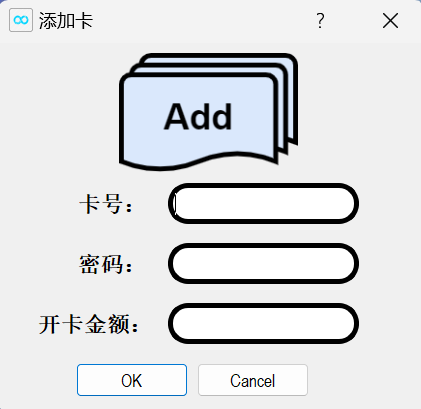
\includegraphics[scale=0.6]{figure/add.png}
        \label{add}
    \end{minipage}
    \begin{figure}[htbp]
        \centering
        \begin{subfigure}{0.24\linewidth}
            \centering
            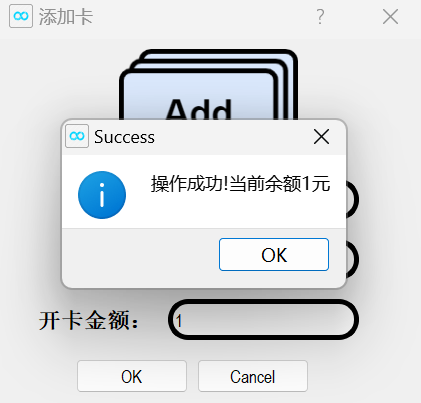
\includegraphics[width=\linewidth]{figure/add_success.png}
            \caption{成功页面}
            \label{add_success}
        \end{subfigure}
        \centering
        \begin{subfigure}{0.24\linewidth}
            \centering
            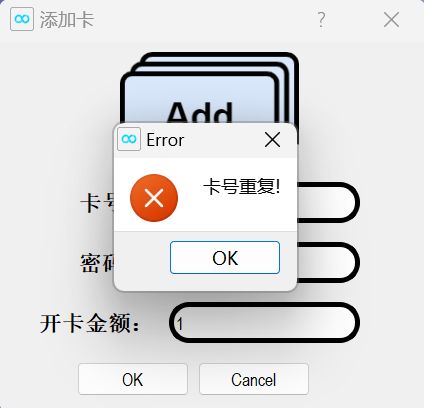
\includegraphics[width=\linewidth]{figure/add_repeat.png}
            \caption{卡号重复页面}
            \label{id_repeat}
        \end{subfigure}
        \centering
        \begin{subfigure}{0.24\linewidth}
            \centering
            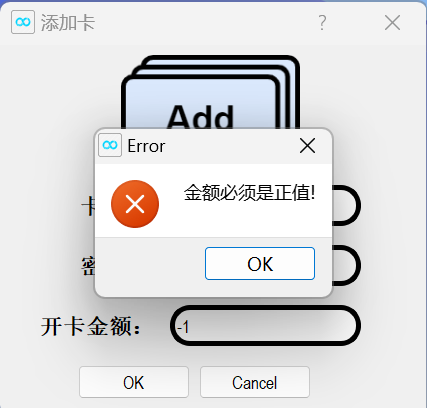
\includegraphics[width=\linewidth]{figure/add_less_zero.png}
            \caption{金额非正页面}
            \label{add_less_zero}
        \end{subfigure}
        \centering
        \begin{subfigure}{0.24\linewidth}
            \centering
            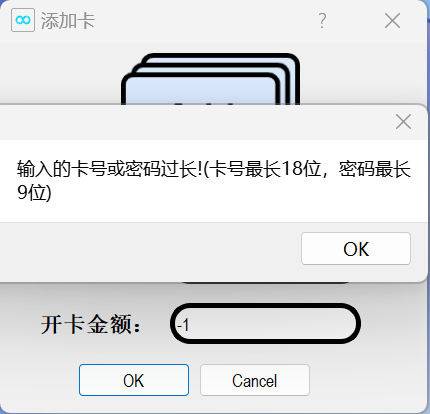
\includegraphics[width=\linewidth]{figure/add_too_long.png}
            \caption{输入过长页面}
            \label{too_long}
        \end{subfigure}
    \end{figure}
    \subsubsection{查询卡}
    \begin{figure}[h]
        \centering
        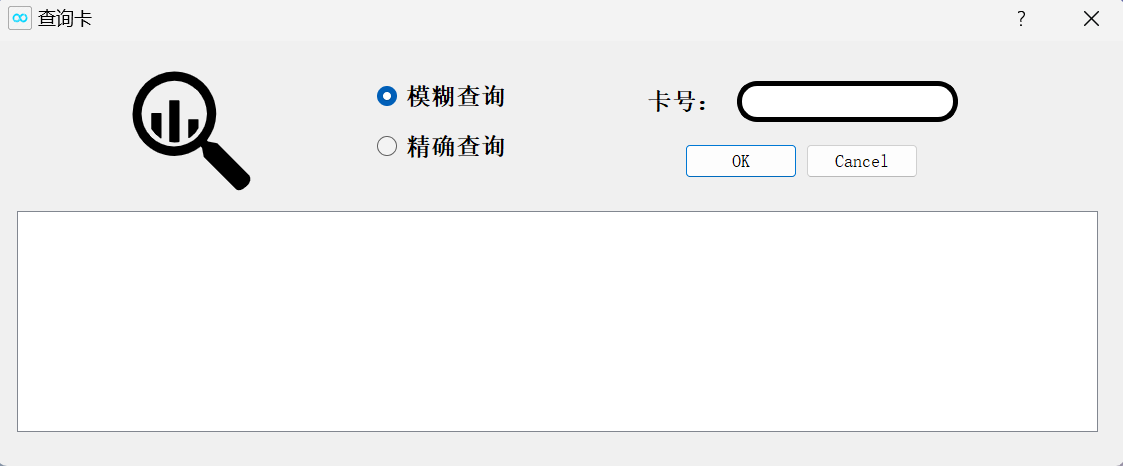
\includegraphics[scale=0.5]{figure/query.png}
        \caption{查询卡}
        \label{query}
    \end{figure}
    \paragraph{功能介绍}
    如\ref{query},用户根据指引输入卡号,通过切换精确与模糊查找找到自己的结果
    \paragraph{返回结果}
    \begin{figure}[h]
        \centering
        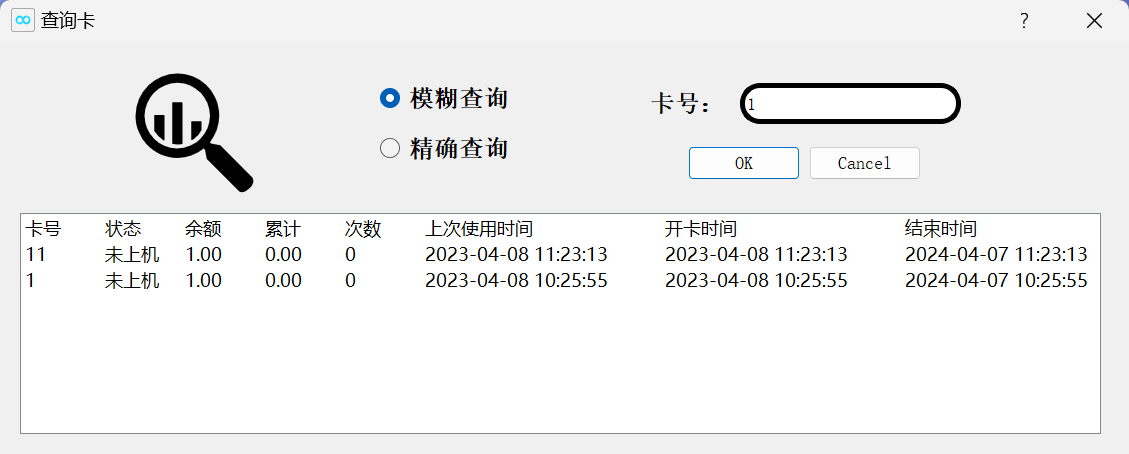
\includegraphics[scale=0.5]{figure/query_big.png}
        \caption{模糊查找}
        \label{query_big}
    \end{figure}
    \begin{figure}[h]
        \centering
        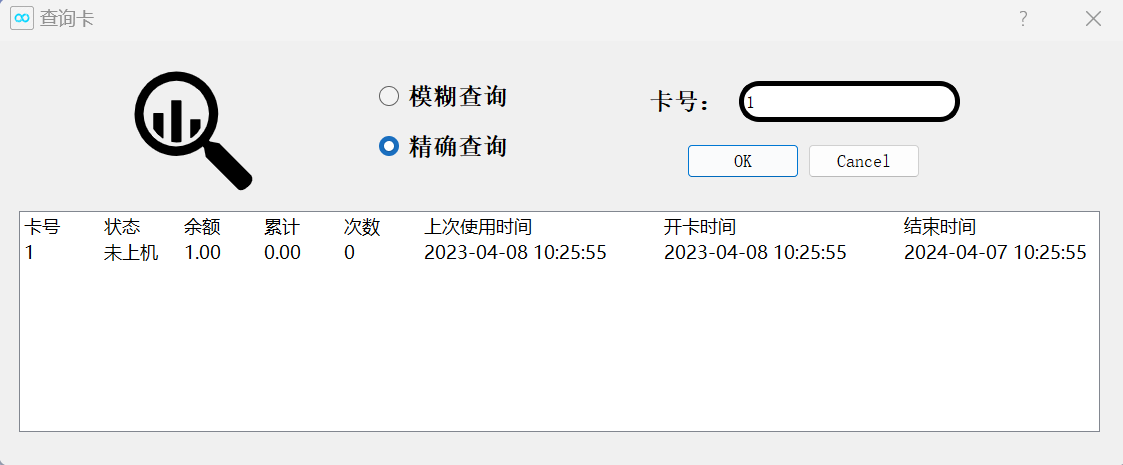
\includegraphics[scale=0.5]{figure/query_small.png}
        \caption{精确查找}
        \label{query_small}
    \end{figure}
    \begin{enumerate}
        \item 模糊查找 如图\ref{query_big},输入较短卡号序列就可以返回所有包含该卡号序列所有卡的信息
        \item 精确查找 如图\ref{query_small},输入精确卡号序列才可以返回该卡的信息
    \end{enumerate}
    \subsubsection{上机}
    \begin{minipage}[h]{0.5\linewidth}
        \paragraph{功能介绍}
        如右图,用户根据指引输入卡号,密码后点击OK就可以上机,该卡会标记为已上机
        \vfill
        \paragraph{返回结果}
        \begin{enumerate}
            \item 成功,则返回\ref{logon_success}
            \item 卡号与密码不匹配页面,则返回\ref{id_password_error}
            \item 已上机再重复上机,则返回\ref{logon_repeat}
            \item 如果该卡金额过少,则返回\ref{logon_less_money}。
        \end{enumerate}
    \end{minipage}
    \begin{minipage}[h]{0.5\linewidth}
        \centering
        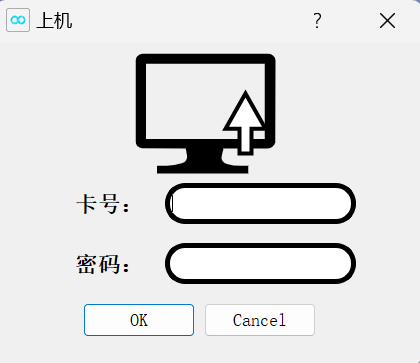
\includegraphics[scale=0.6]{figure/logon.png}
        \label{logon}
    \end{minipage}
    \begin{figure}[htbp]
        \centering
        \begin{subfigure}{0.24\linewidth}
            \centering
            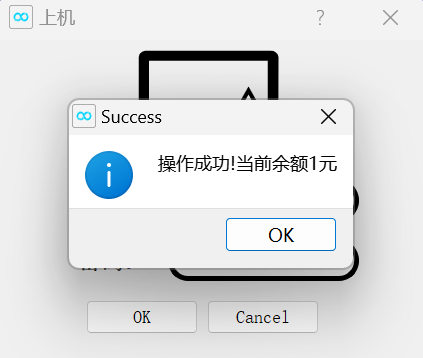
\includegraphics[width=\linewidth]{figure/logon_success.png}
            \caption{成功页面}
            \label{logon_success}
        \end{subfigure}
        \centering
        \begin{subfigure}{0.24\linewidth}
            \centering
            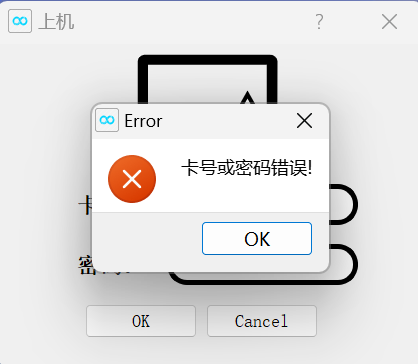
\includegraphics[width=\linewidth]{figure/logon_password_error.png}
            \caption{卡号与密码不匹配页面}
            \label{id_password_error}
        \end{subfigure}
        \centering
        \begin{subfigure}{0.24\linewidth}
            \centering
            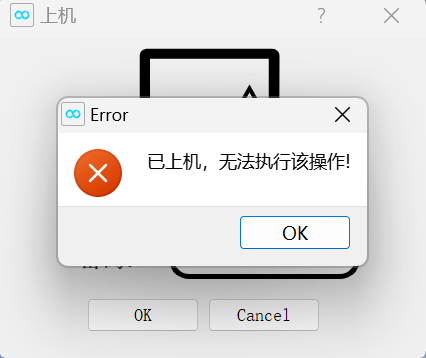
\includegraphics[width=\linewidth]{figure/logon_two.png}
            \caption{重复上机}
            \label{logon_repeat}
        \end{subfigure}
        \centering
        \begin{subfigure}{0.24\linewidth}
            \centering
            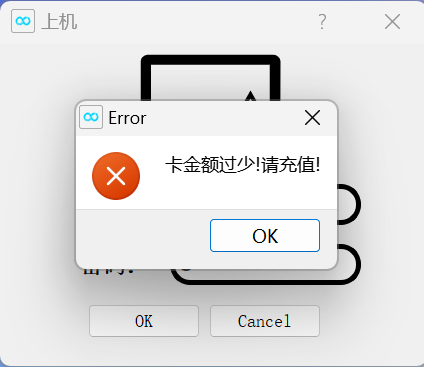
\includegraphics[width=\linewidth]{figure/logon_less_money.png}
            \caption{上机余额过少}
            \label{logon_less_money}
        \end{subfigure}
    \end{figure}
    \subsubsection{下机}
    \begin{minipage}[h]{0.5\linewidth}
        \paragraph{功能介绍}
        如右图,用户根据指引输入卡号,密码后点击OK就可以下机,下机时该卡会标记为已下机,
        同时扣除费用。
        \vfill
        \paragraph{返回结果}
        \begin{enumerate}
            \item 成功,则返回\ref{settle_success},提示下机后的余额
            \item 卡号与密码不匹配页面,则返回\ref{settle_id_password_error}
            \item 已下机再重复下机,则返回\ref{settle_repeat}
            \item 如果该卡金额过少,则返回\ref{settle_less_money}。
        \end{enumerate}
    \end{minipage}
    \begin{minipage}[h]{0.5\linewidth}
        \centering
        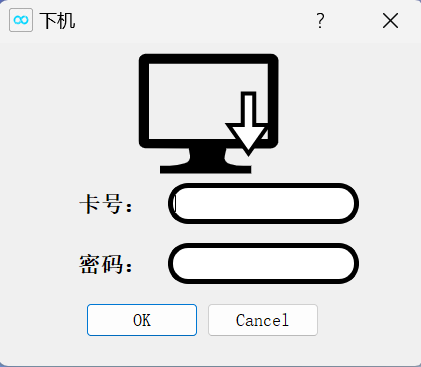
\includegraphics[scale=0.6]{figure/settle.png}
        \label{settle}
    \end{minipage}
    \begin{figure}[htbp]
        \centering
        \begin{subfigure}{0.24\linewidth}
            \centering
            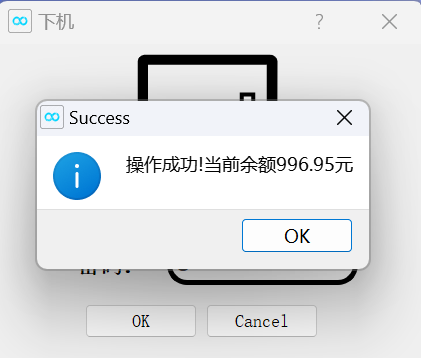
\includegraphics[width=\linewidth]{figure/settle_success.png}
            \caption{成功页面}
            \label{settle_success}
        \end{subfigure}
        \centering
        \begin{subfigure}{0.24\linewidth}
            \centering
            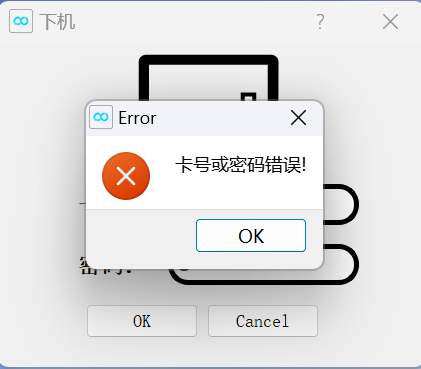
\includegraphics[width=\linewidth]{figure/settle_id_password_error.png}
            \caption{卡号与密码不匹配页面}
            \label{settle_id_password_error}
        \end{subfigure}
        \centering
        \begin{subfigure}{0.24\linewidth}
            \centering
            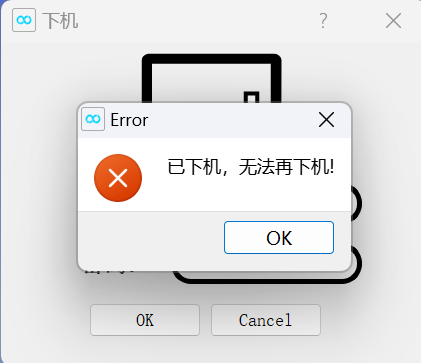
\includegraphics[width=\linewidth]{figure/settle_repeat.png}
            \caption{重复下机}
            \label{settle_repeat}
        \end{subfigure}
        \centering
        \begin{subfigure}{0.24\linewidth}
            \centering
            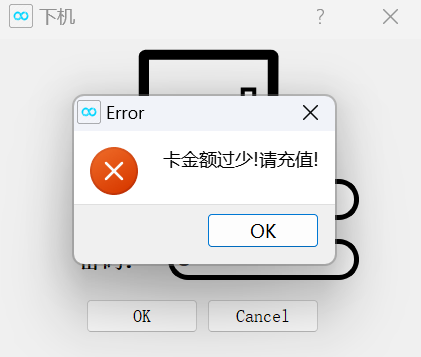
\includegraphics[width=\linewidth]{figure/settle_less_money.png}
            \caption{下机余额过少}
            \label{settle_less_money}
        \end{subfigure}
    \end{figure}
    \subsubsection{充值}
    \begin{minipage}[h]{0.5\linewidth}
        \paragraph{功能介绍}
        如右图,用户根据指引输入卡号,
        密码,充值金额后点击OK就可以充值.
        \vfill
        \paragraph{返回结果}
        \begin{enumerate}
            \item 成功,则返回\ref{addmoney_success}
            \item 卡号与密码不匹配,则返回\ref{addmeny_id_password_error}
            \item 输入充值金额非正,则返回\ref{addmoney_less_zero}
            \item 输入卡号或密码过长,则返回\ref{addmoney_too_long}。
        \end{enumerate}
    \end{minipage}
    \begin{minipage}[h]{0.5\linewidth}
        \centering
        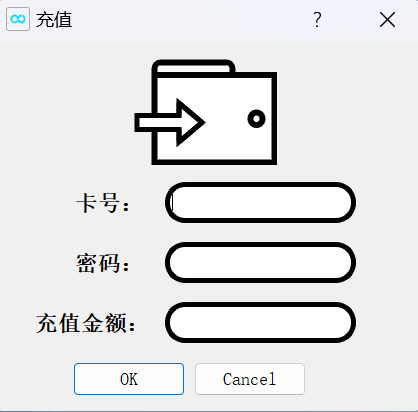
\includegraphics[scale=0.6]{figure/addmoney.png}
        \label{addmoney}
    \end{minipage}
    \begin{figure}[htbp]
        \centering
        \begin{subfigure}{0.24\linewidth}
            \centering
            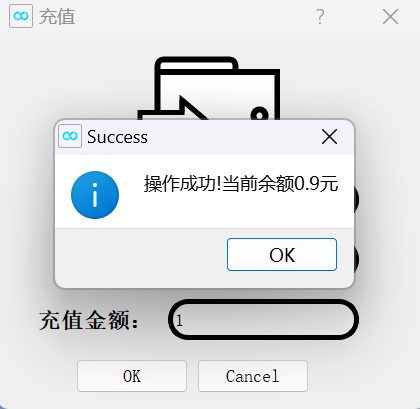
\includegraphics[width=\linewidth]{figure/addmoney_success.png}
            \caption{成功页面}
            \label{addmoney_success}
        \end{subfigure}
        \centering
        \begin{subfigure}{0.24\linewidth}
            \centering
            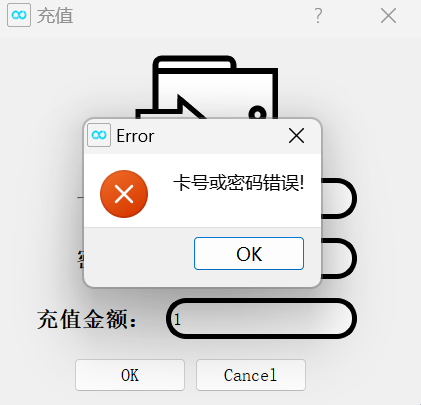
\includegraphics[width=\linewidth]{figure/addmoney_id_password_error.png}
            \caption{卡号与密码不匹配页面}
            \label{addmeny_id_password_error}
        \end{subfigure}
        \centering
        \begin{subfigure}{0.24\linewidth}
            \centering
            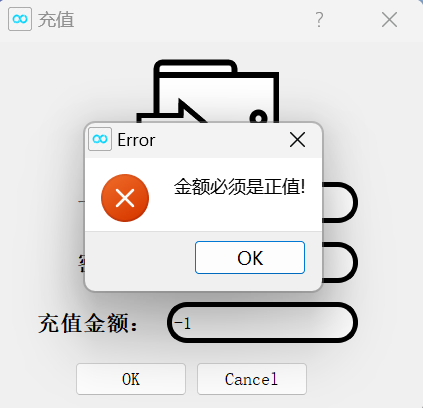
\includegraphics[width=\linewidth]{figure/addmoney_less _zero.png}
            \caption{金额非正页面}
            \label{addmoney_less_zero}
        \end{subfigure}
        \centering
        \begin{subfigure}{0.24\linewidth}
            \centering
            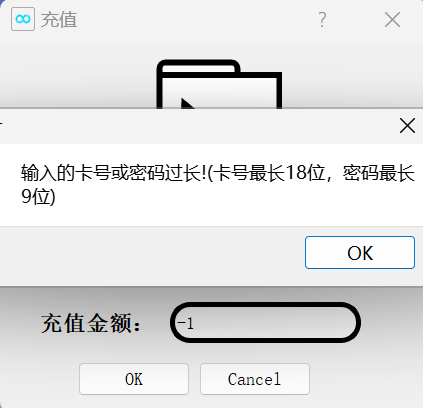
\includegraphics[width=\linewidth]{figure/addmoney_too_long.png}
            \caption{输入过长页面}
            \label{addmoney_too_long}
        \end{subfigure}
    \end{figure}
    \subsubsection{退款}
    \begin{minipage}[h]{0.5\linewidth}
        \paragraph{功能介绍}
        如右图,用户根据指引输入卡号,
        密码,退款金额后点击OK就可以退款.
        \vfill
        \paragraph{返回结果}
        \begin{enumerate}
            \item 成功,则返回\ref{refund_success}
            \item 卡号与密码不匹配,则返回\ref{refund_id_password_error}
            \item 输入退款金额非正,则返回\ref{refund_less_zero}
            \item 退款金额不足,则返回\ref{refund_less_money}
        \end{enumerate}
    \end{minipage}
    \begin{minipage}[h]{0.5\linewidth}
        \centering
        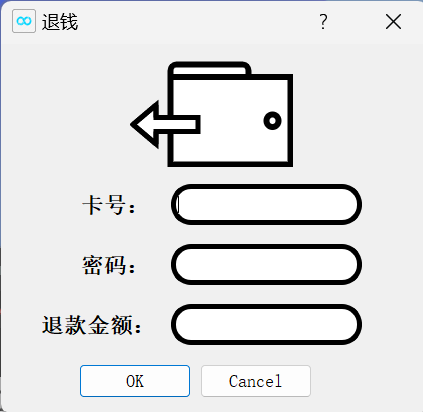
\includegraphics[scale=0.6]{figure/refund.png}
        \label{refund}
    \end{minipage}
    \begin{figure}[htbp]
        \centering
        \begin{subfigure}{0.24\linewidth}
            \centering
            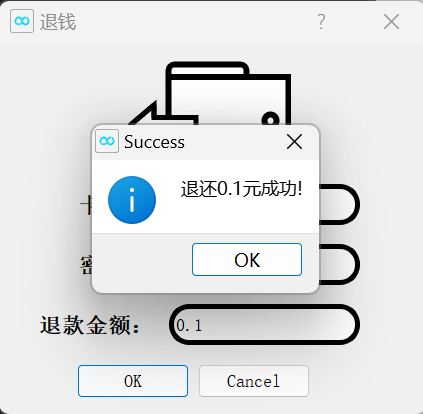
\includegraphics[width=\linewidth]{figure/refund_success.png}
            \caption{成功页面}
            \label{refund_success}
        \end{subfigure}
        \centering
        \begin{subfigure}{0.24\linewidth}
            \centering
            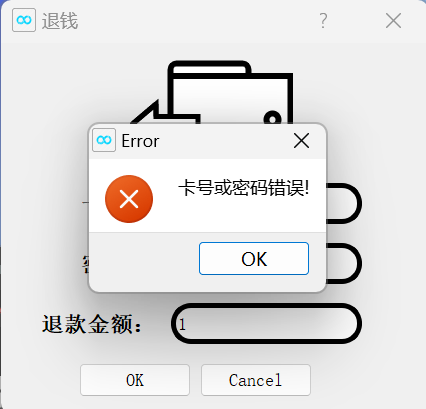
\includegraphics[width=\linewidth]{figure/refund_id_password_error.png}
            \caption{卡号与密码不匹配页面}
            \label{refund_id_password_error}
        \end{subfigure}
        \centering
        \begin{subfigure}{0.24\linewidth}
            \centering
            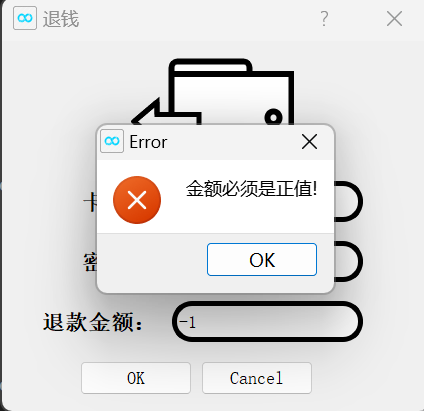
\includegraphics[width=\linewidth]{figure/refund_less_zero.png}
            \caption{金额非正页面}
            \label{refund_less_zero}
        \end{subfigure}
        \centering
        \begin{subfigure}{0.24\linewidth}
            \centering
            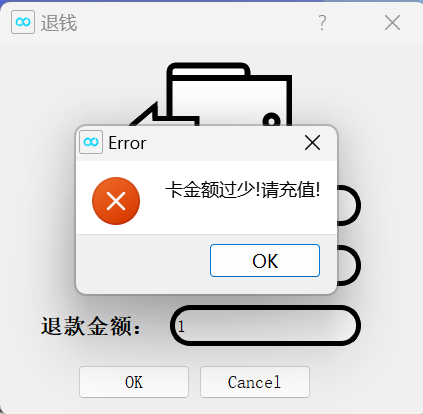
\includegraphics[width=\linewidth]{figure/refund_less_money.png}
            \caption{退款金额不足}
            \label{refund_less_money}
        \end{subfigure}
    \end{figure}
    \subsubsection{注销}
    \begin{minipage}[h]{0.5\linewidth}
        \paragraph{功能介绍}
        如右图,用户根据指引输入卡号,
        密码后点击OK就可以注销该卡.
        \vfill
        \paragraph{返回结果}
        \begin{enumerate}
            \item 成功,则返回\ref{annul_success}
            \item 卡号与密码不匹配,则返回\ref{annul_id_password_error}
            \item 注销时处于上机状态,则返回\ref{annul_logon_error}
            \item 注销时金额过少,则返回\ref{annul_less_money}
        \end{enumerate}
    \end{minipage}
    \begin{minipage}[h]{0.5\linewidth}
        \centering
        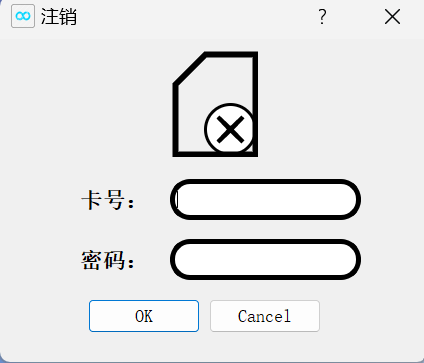
\includegraphics[scale=0.6]{figure/annul.png}
        \label{annul}
    \end{minipage}
    \begin{figure}[htbp]
        \centering
        \begin{subfigure}{0.24\linewidth}
            \centering
            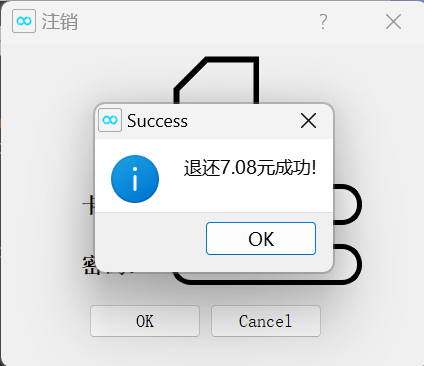
\includegraphics[width=\linewidth]{figure/annul_success.png}
            \caption{成功页面}
            \label{annul_success}
        \end{subfigure}
        \centering
        \begin{subfigure}{0.24\linewidth}
            \centering
            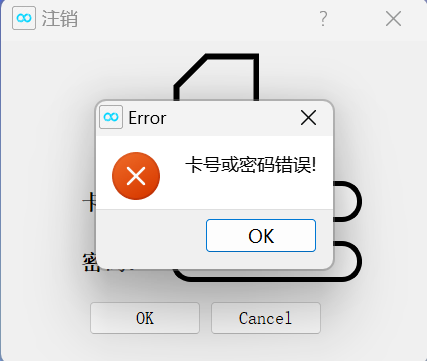
\includegraphics[width=\linewidth]{figure/annul_id_password_error.png}
            \caption{卡号与密码不匹配页面}
            \label{annul_id_password_error}
        \end{subfigure}
        \centering
        \begin{subfigure}{0.24\linewidth}
            \centering
            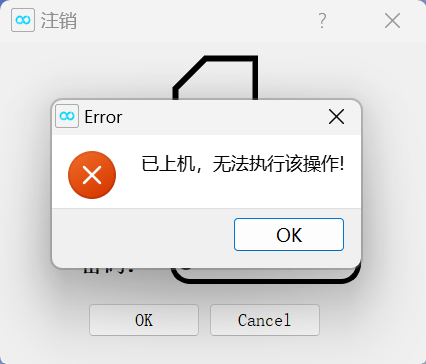
\includegraphics[width=\linewidth]{figure/annul_logon_error.png}
            \caption{注销时处于上机}
            \label{annul_logon_error}
        \end{subfigure}
        \centering
        \begin{subfigure}{0.24\linewidth}
            \centering
            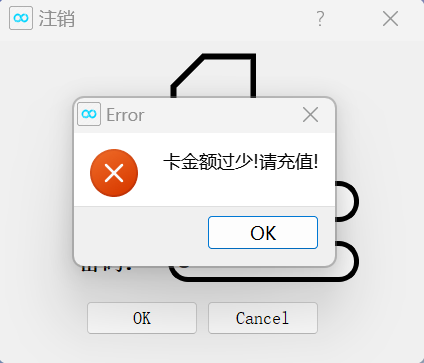
\includegraphics[width=\linewidth]{figure/annul_less_money.png}
            \caption{注销时金额小于0}
            \label{annul_less_money}
        \end{subfigure}
    \end{figure}
    \subsubsection{可以进行保存文件}
    \begin{minipage}[h]{0.5\linewidth}
        \paragraph{功能介绍}
        如右图,每次操作后,会自动生成card.ams与billing.ams文件,
        两个文件为二进制文件 
    \end{minipage}
    \begin{minipage}[h]{0.5\linewidth}
        \centering
        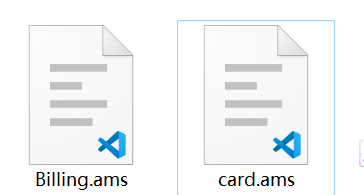
\includegraphics[scale=0.6]{figure/file.png}
        \label{annul}
    \end{minipage}
    \subsection{拓展功能}
    \subsubsection{权限管理}
    \begin{minipage}[h]{0.5\linewidth}
        \paragraph{功能介绍}
        如右图,统计服务必须得到管理员权限,账号,密码写在global.h文件,账号默认为NaCl,密码为qwert12345.
        \vfill
        \paragraph{返回结果}
        \begin{enumerate}
            \item 成功,则返回\ref{admin_success}
            \item 帐号与密码不匹配,则返回\ref{admin_id_password_error}
        \end{enumerate}
    \end{minipage}
    \begin{minipage}[h]{0.45\linewidth}
        \centering
        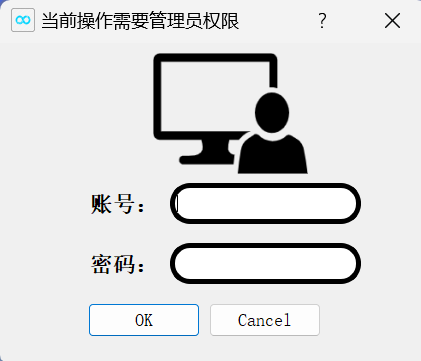
\includegraphics[scale=0.6]{figure/admin.png}
        \label{admin}
    \end{minipage}
    \begin{figure}[htbp]
        \centering
        \begin{subfigure}{0.45\linewidth}
            \centering
            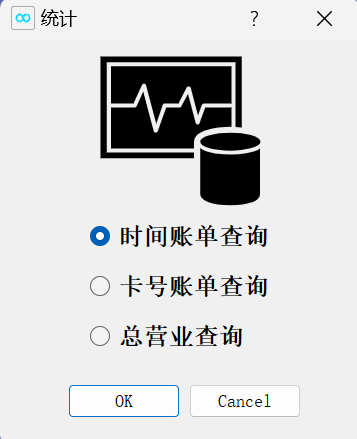
\includegraphics[scale=0.5]{figure/count.png}
            \caption{成功页面}
            \label{admin_success}
        \end{subfigure}
        \centering
        \begin{subfigure}{0.5\linewidth}
            \centering
            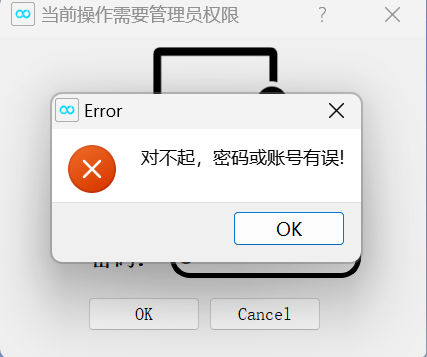
\includegraphics[scale=0.5]{figure/admin_error.png}
            \caption{帐号与密码不匹配页面}
            \label{admin_id_password_error}
        \end{subfigure}
    \end{figure}
    \subsubsection{统计}
    \begin{minipage}[h]{0.5\linewidth}
        \paragraph{功能介绍}
        如右图,为统计提供三种统计
        \vfill
        \paragraph{返回结果}
        \begin{enumerate}
            \item 如\ref{count_time},按时间节点统计消费记录
            \item 如\ref{count_card},按卡号统计统计消费记录
            \item 如\ref{count_total},总金额统计
        \end{enumerate}
    \end{minipage}
    \begin{minipage}[h]{0.45\linewidth}
        \centering
        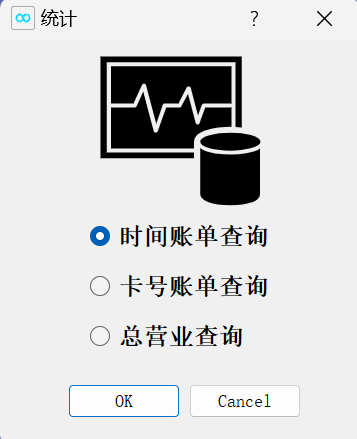
\includegraphics[scale=0.5]{figure/count.png}
        \label{count}
    \end{minipage}
    \begin{figure}[htbp]
        \centering
        \begin{subfigure}{0.3\linewidth}
            \centering
            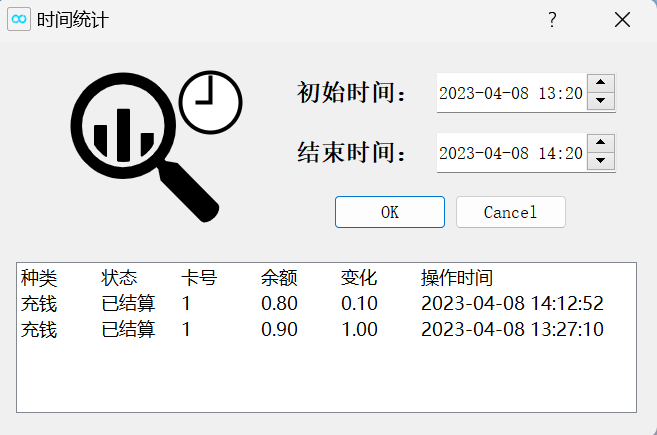
\includegraphics[scale=0.4]{figure/count_time.png}
            \caption{按时间统计}
            \label{count_time}
        \end{subfigure}
        \centering
        \begin{subfigure}{0.3\linewidth}
            \centering
            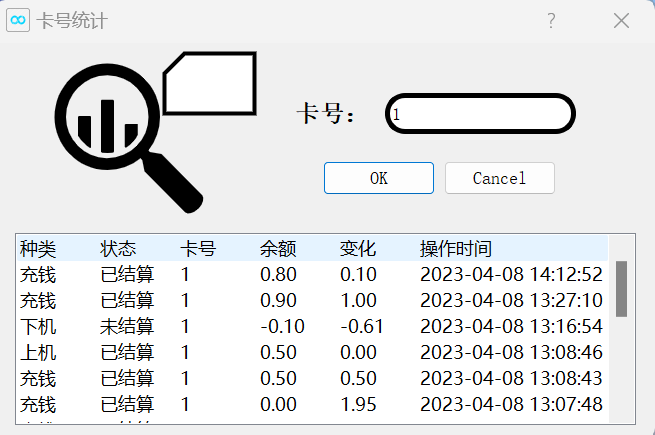
\includegraphics[scale=0.4]{figure/count_card.png}
            \caption{按卡号统计}
            \label{count_card}
        \end{subfigure}
        \centering
        \begin{subfigure}{0.3\linewidth}
            \centering
            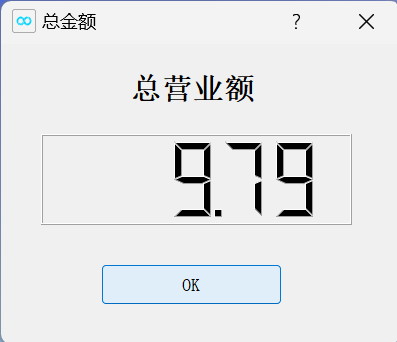
\includegraphics[scale=0.5]{figure/count_total.png}
            \caption{总金额统计}
            \label{count_total}
        \end{subfigure}
    \end{figure}
    \subsubsection{定时启动页面}
    \begin{minipage}[h]{0.45\linewidth}
        \paragraph{功能介绍}
            点下程序后会有个2s的启动页面展示,该窗口可以自由拖动,四周使用圆角,更加美观。
    \end{minipage}
    \begin{minipage}[h]{0.45\linewidth}
        \centering
        
\includegraphics[scale=0.5]{figure/welcome.png}
    \end{minipage}
    \subsubsection{采用图形页面}
    \begin{enumerate}
        \item 相比CLI程序,更加美观,更加方便用户操作
        \item 该程序使用了Qt进行GUI编写,支持Windows,Linux跨平台运行
    \end{enumerate}
    \section{典型算法分析}
    \subsection{添加卡流程分析}
    \begin{figure}[h]
        \centering
        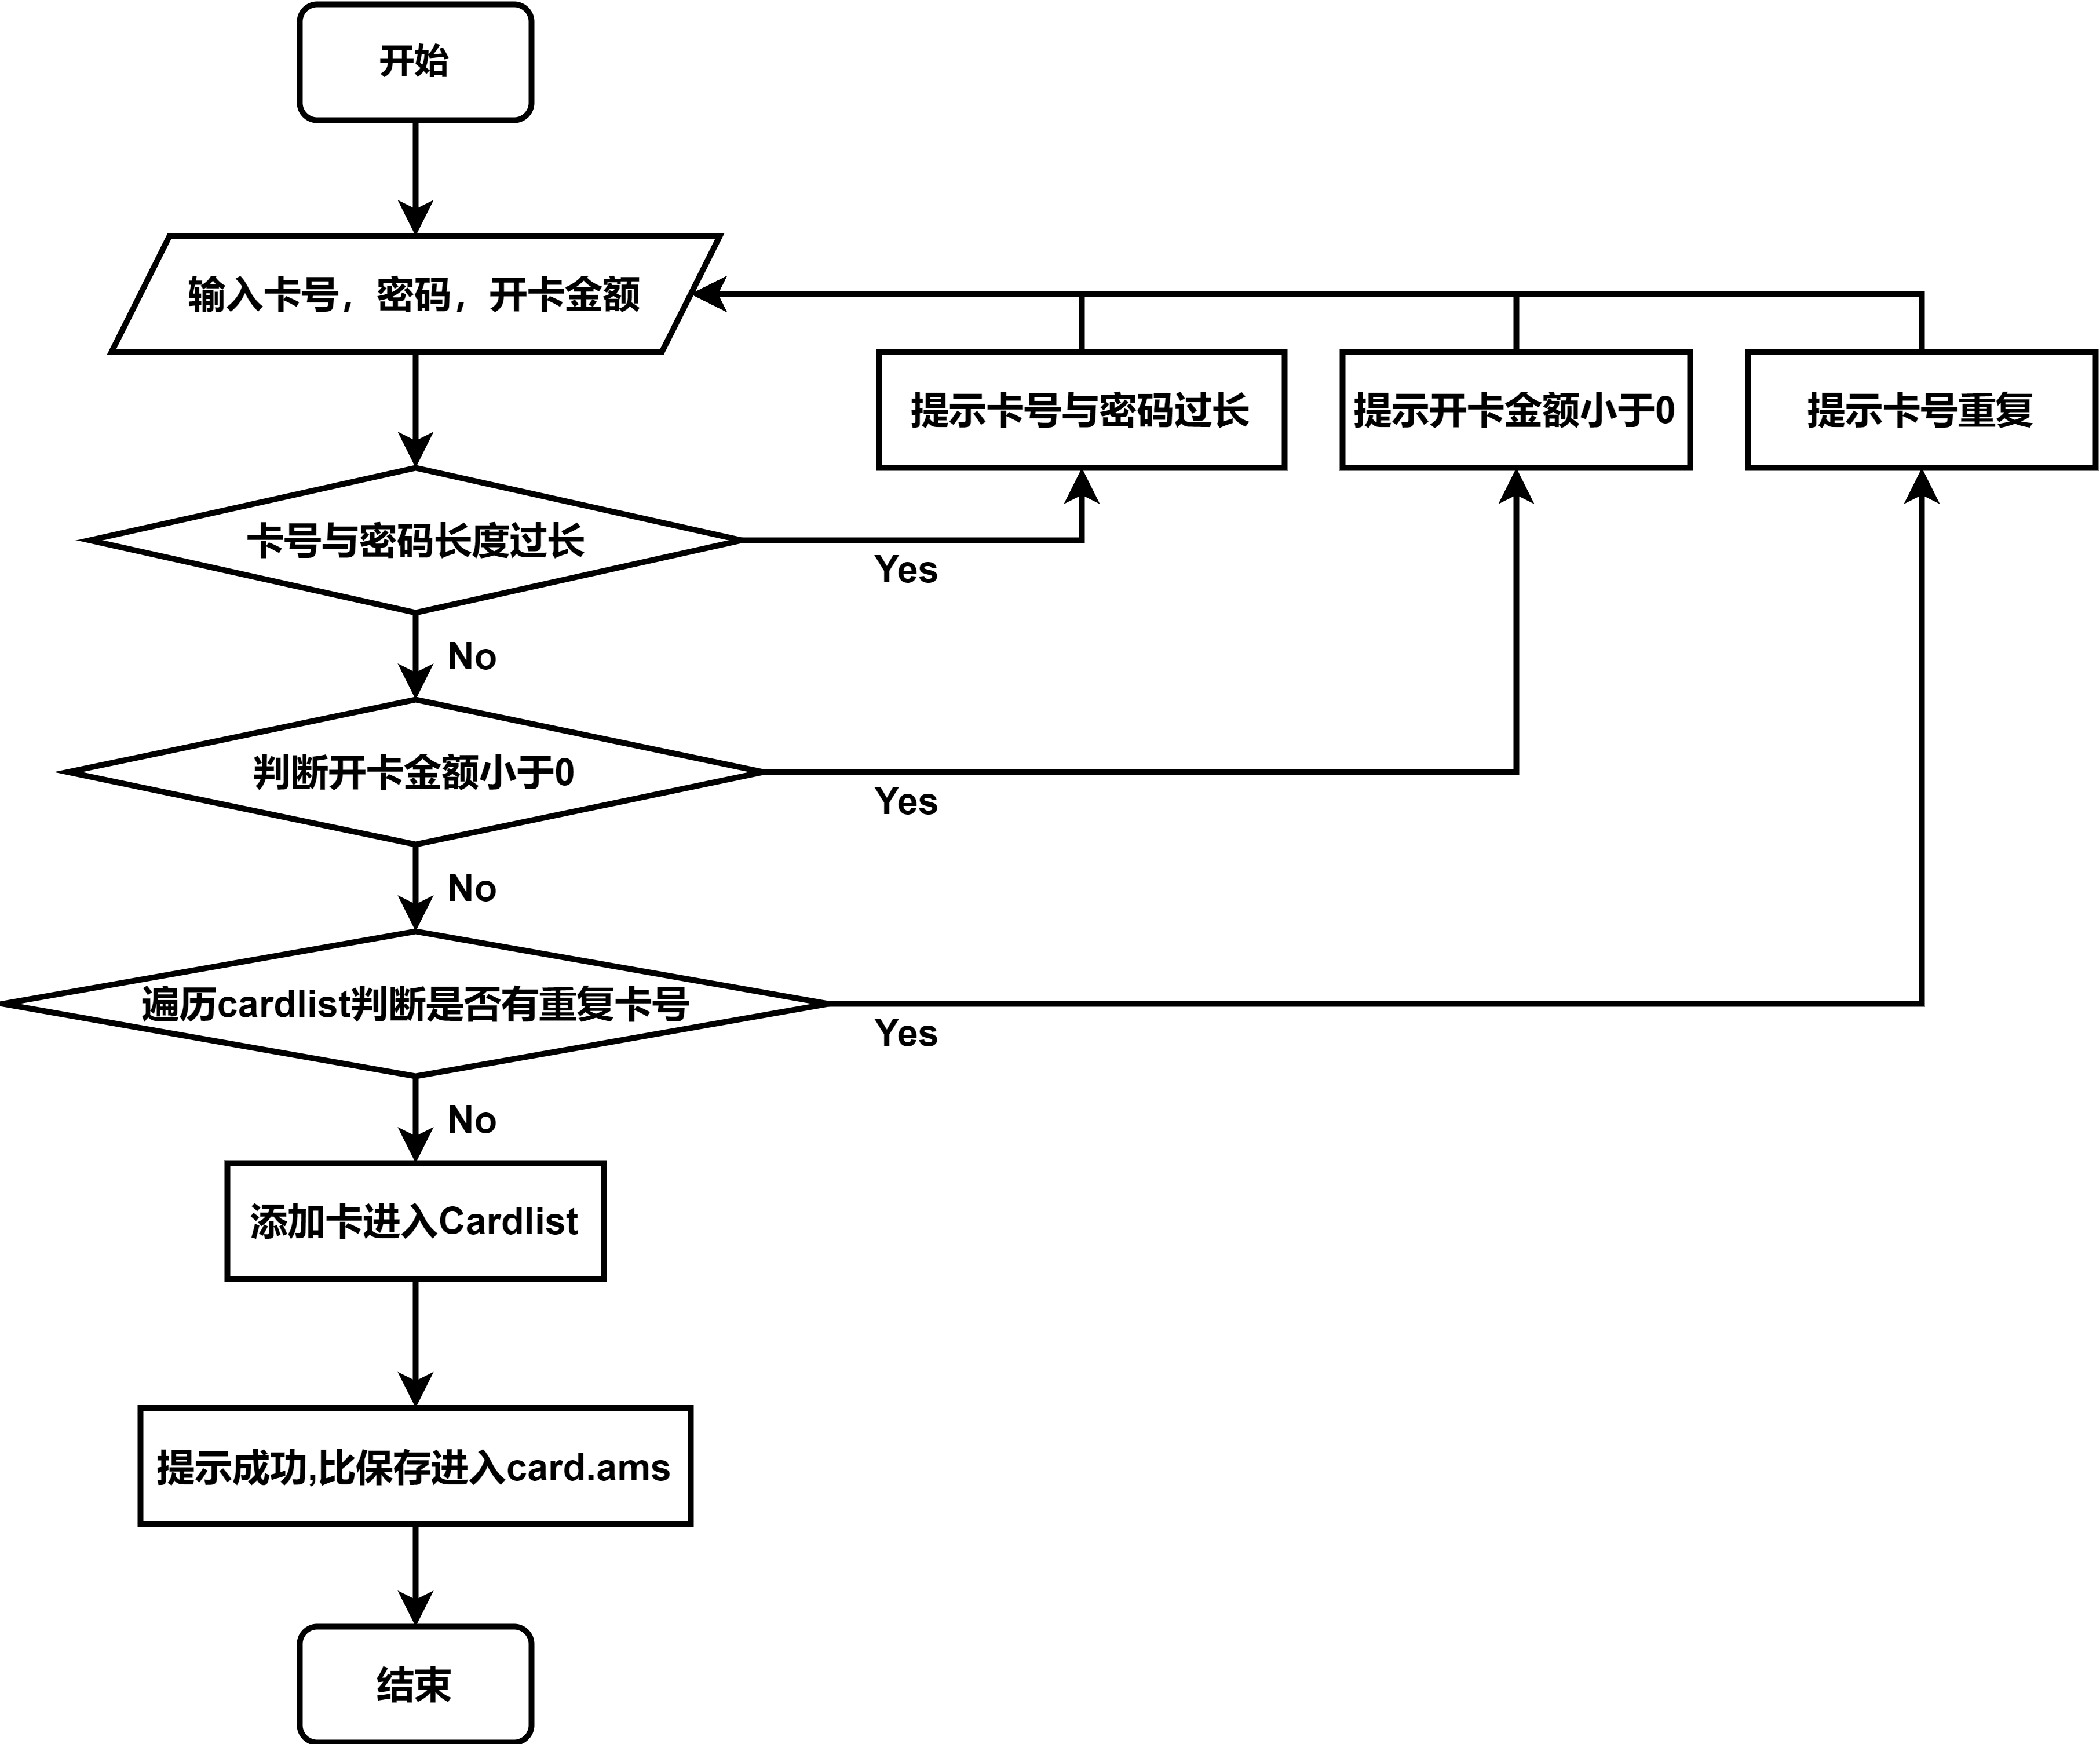
\includegraphics[scale=0.14]{figure/add_pic.png}
        \caption{添加卡流程图}
        \label{add_pic}
    \end{figure}
    如图\ref{add_pic}为添加卡的流程图,首先判断是否存在输入非数字,长度过长问题,然后链表链表cardlist判断是否有重复卡号,
    这些处理通过后才能完成添加卡,并保存到card.ams,这些处理提高了软件的鲁棒性,防止意外输出导致程序出错。
    \subsection{统计流程分析}
    \begin{figure}[h]
        \centering
        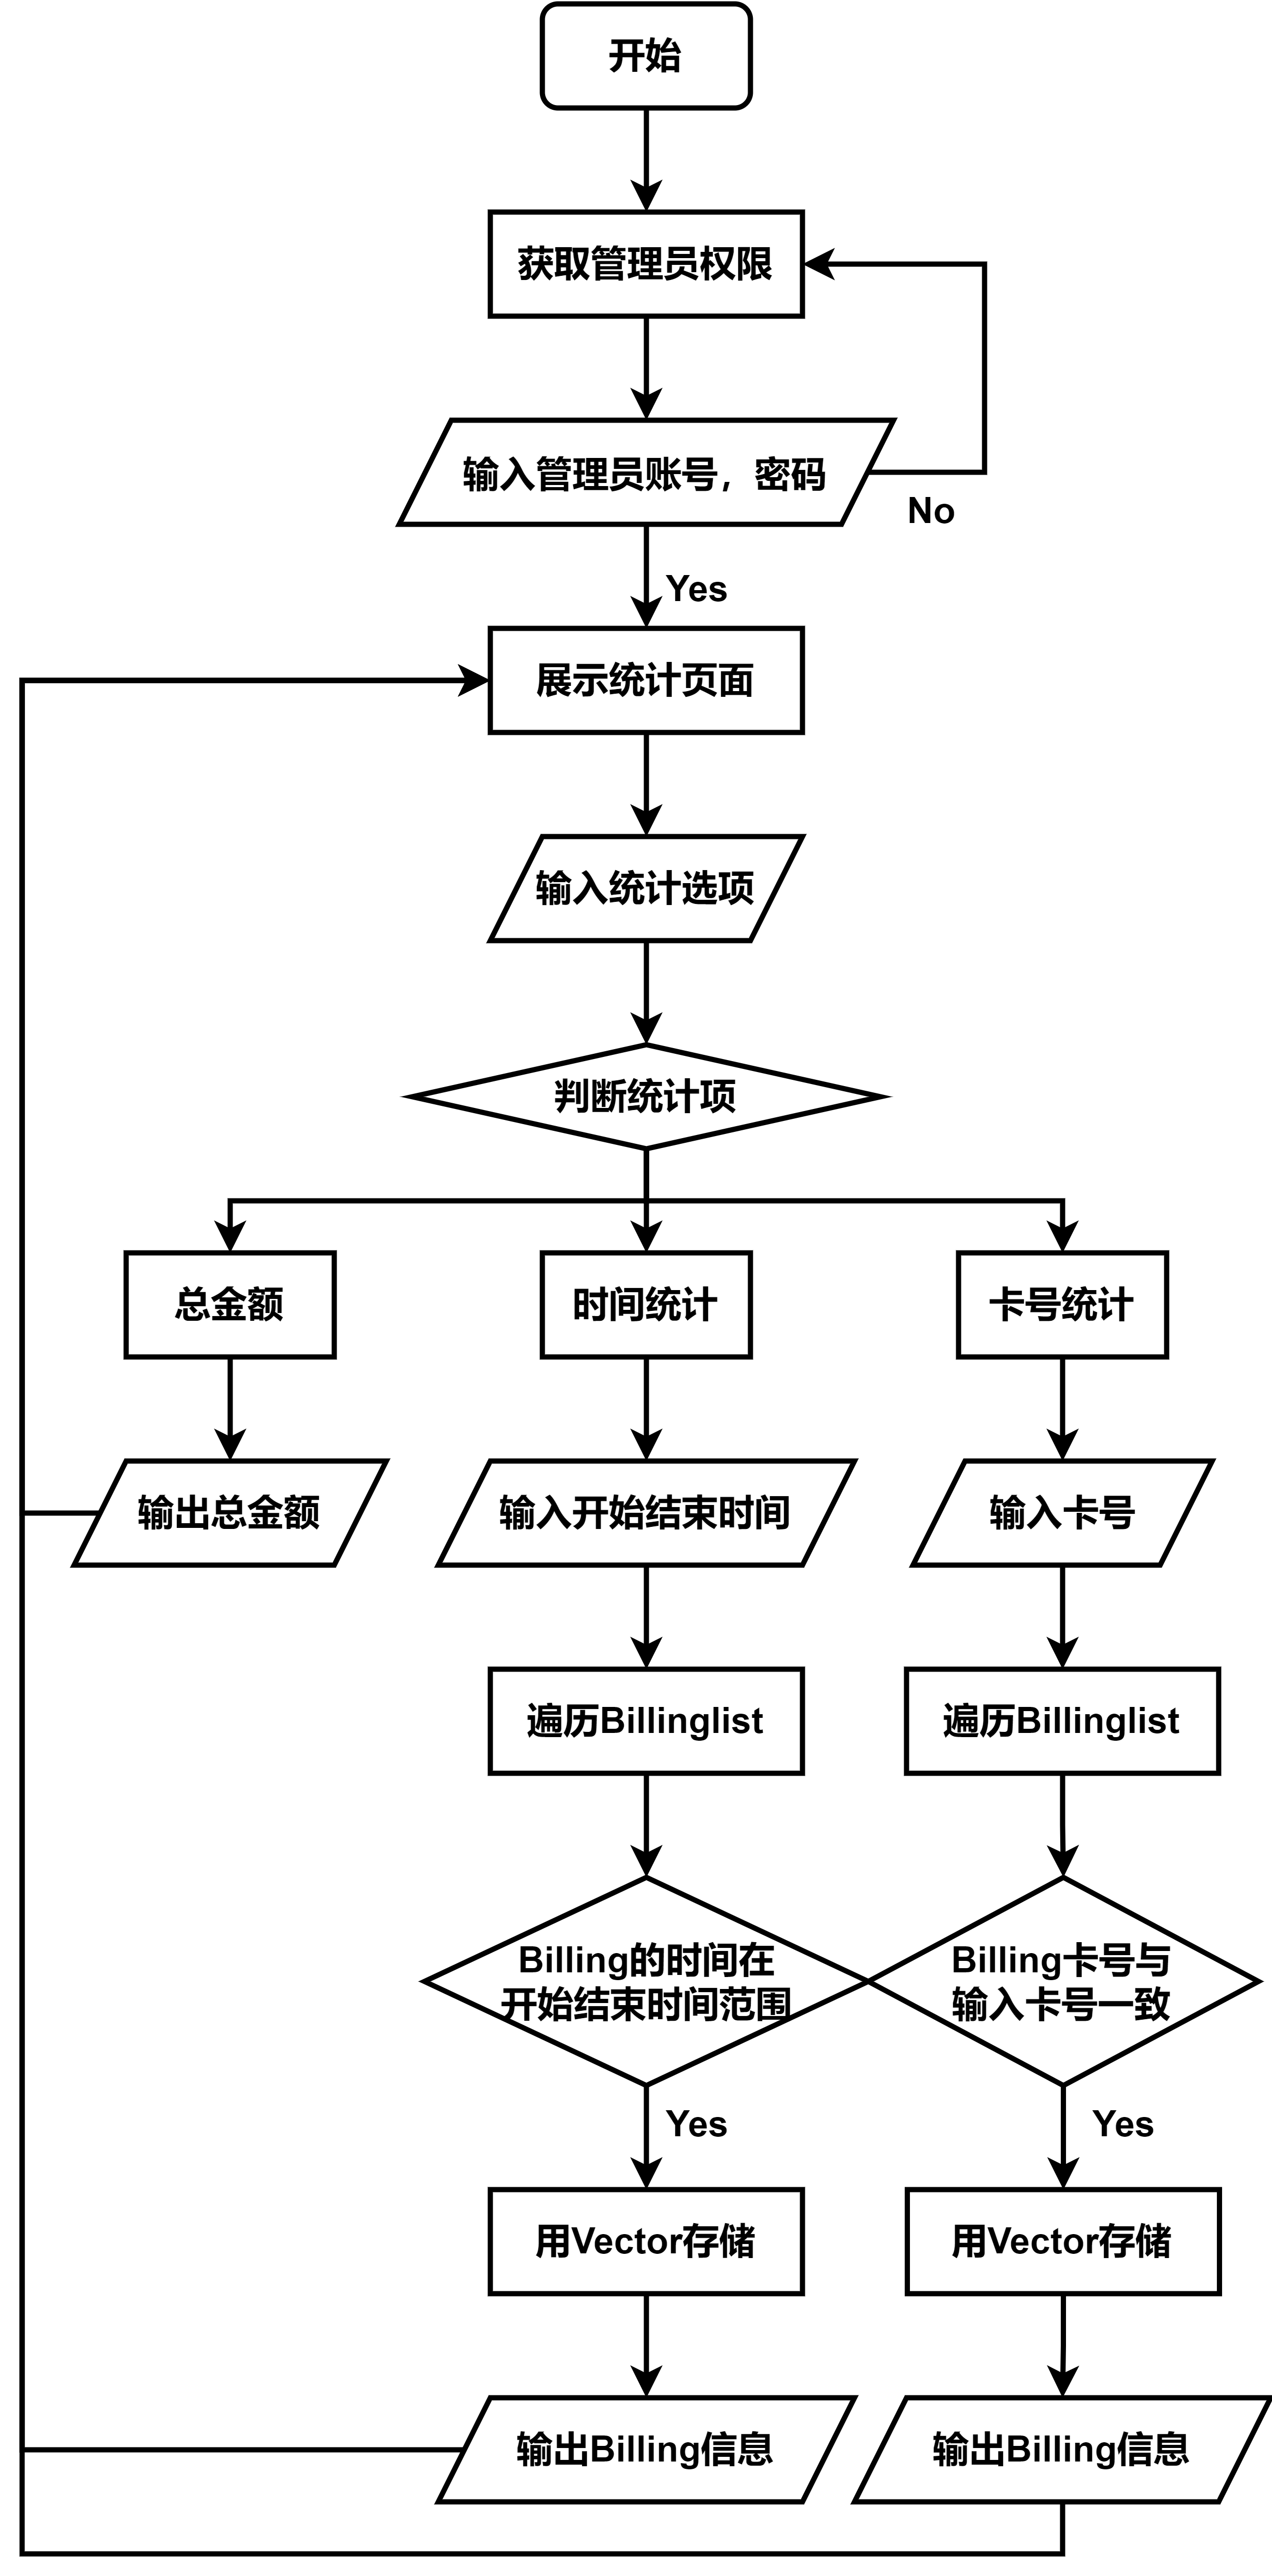
\includegraphics[scale=0.09]{figure/count_pic.png}
        \caption{统计流程图}
        \label{count_pic}
    \end{figure}
    如图\ref{count_pic}为统计的流程图,首先获取管理员权限,再进入统计页面,选择所需功能,如果是按时间统计,则输入开始结束时间后
    ,通过遍历Billinglist,如果Billing的时间在其之内,则通过Billing.tostring()函数转换成string,再存放在vector<string>内,
    最后将vector<string>内容输出,如果是按卡号统计,如果Billing的卡号与输入相等,转换成string,存入vector<string>输出,如果是
    总金额统计,则直接输出总盈利金额。
    \newpage
    \subsection{上机流程分析}
    \begin{figure}[h]
        \centering
        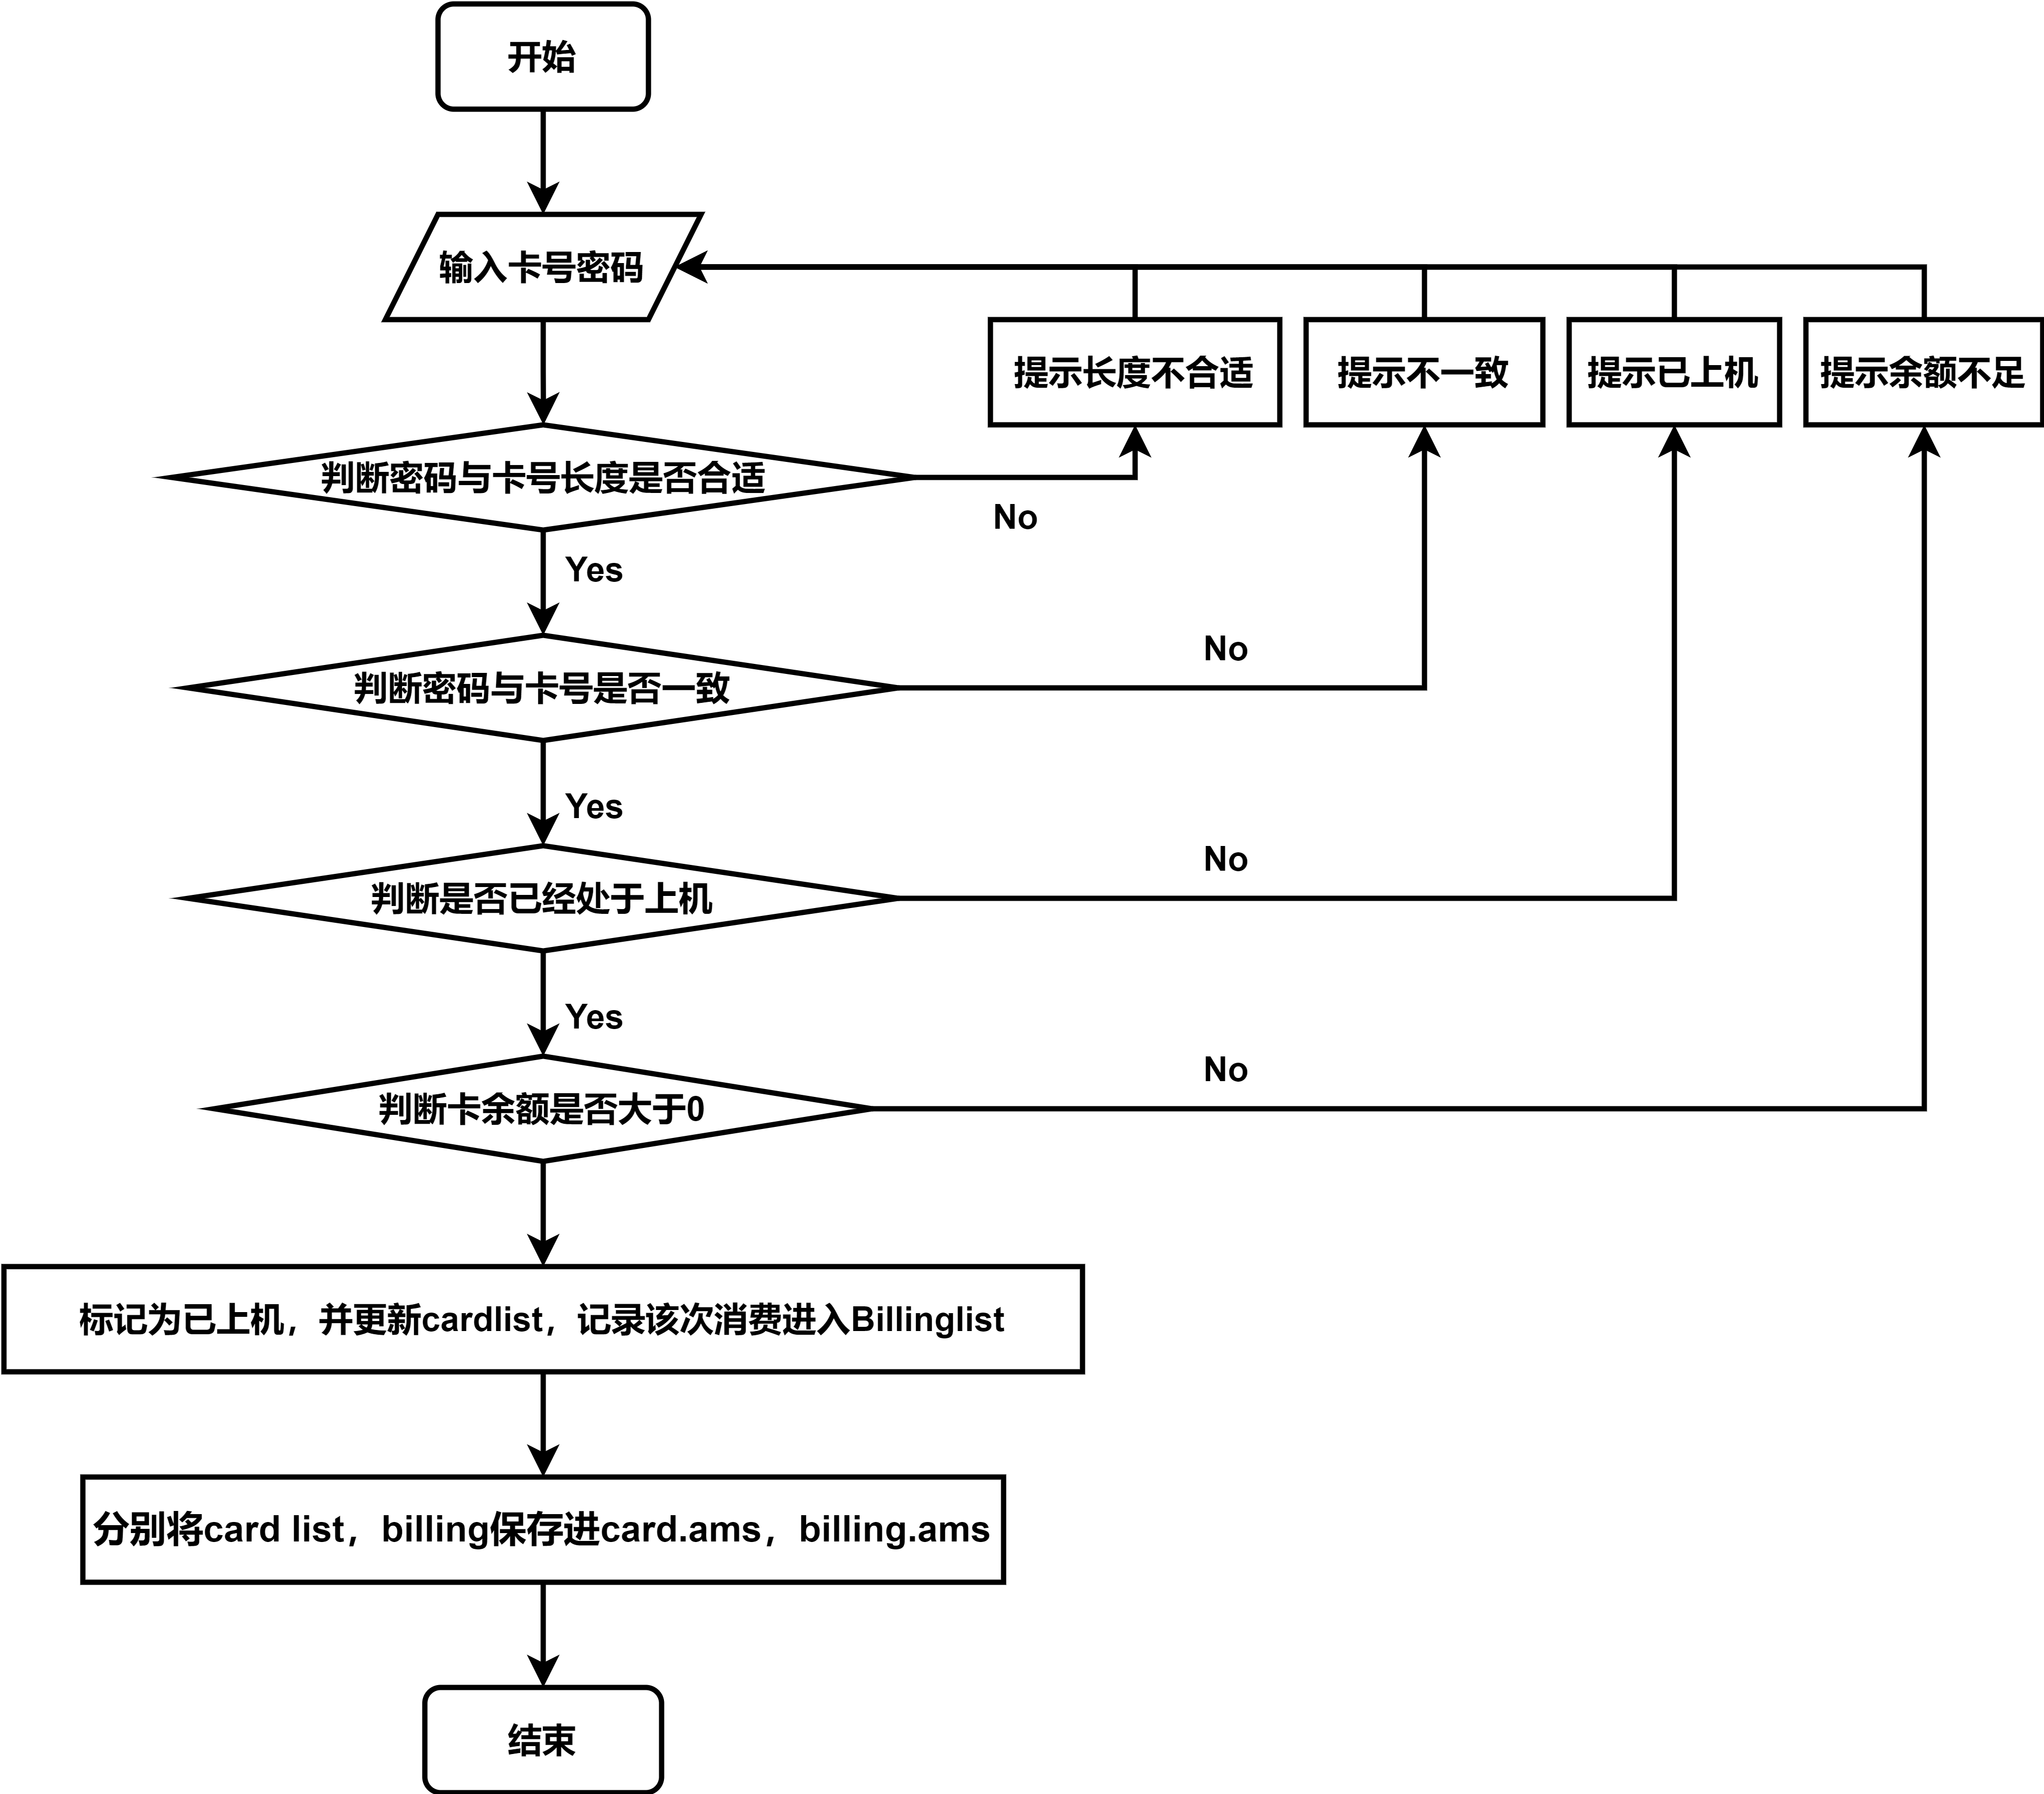
\includegraphics[scale=0.115]{figure/logon_pic.png}
        \caption{上机流程图}
        \label{logon_pic}
    \end{figure}
    如图\ref{logon_pic}为上机的流程图,首先判断是否存在输入长度过长问题,然后遍历链表cardlist判断是否该卡是否存在,该卡密码是否正确,
    再判断是否已经处于下机状态,是否金额足够,通过后把该卡标记为上机,并分别保存卡信息与消费到card.ams,billing.ams.
    \newpage
    \subsection{下机流程分析}
    \begin{figure}[h]
        \centering
        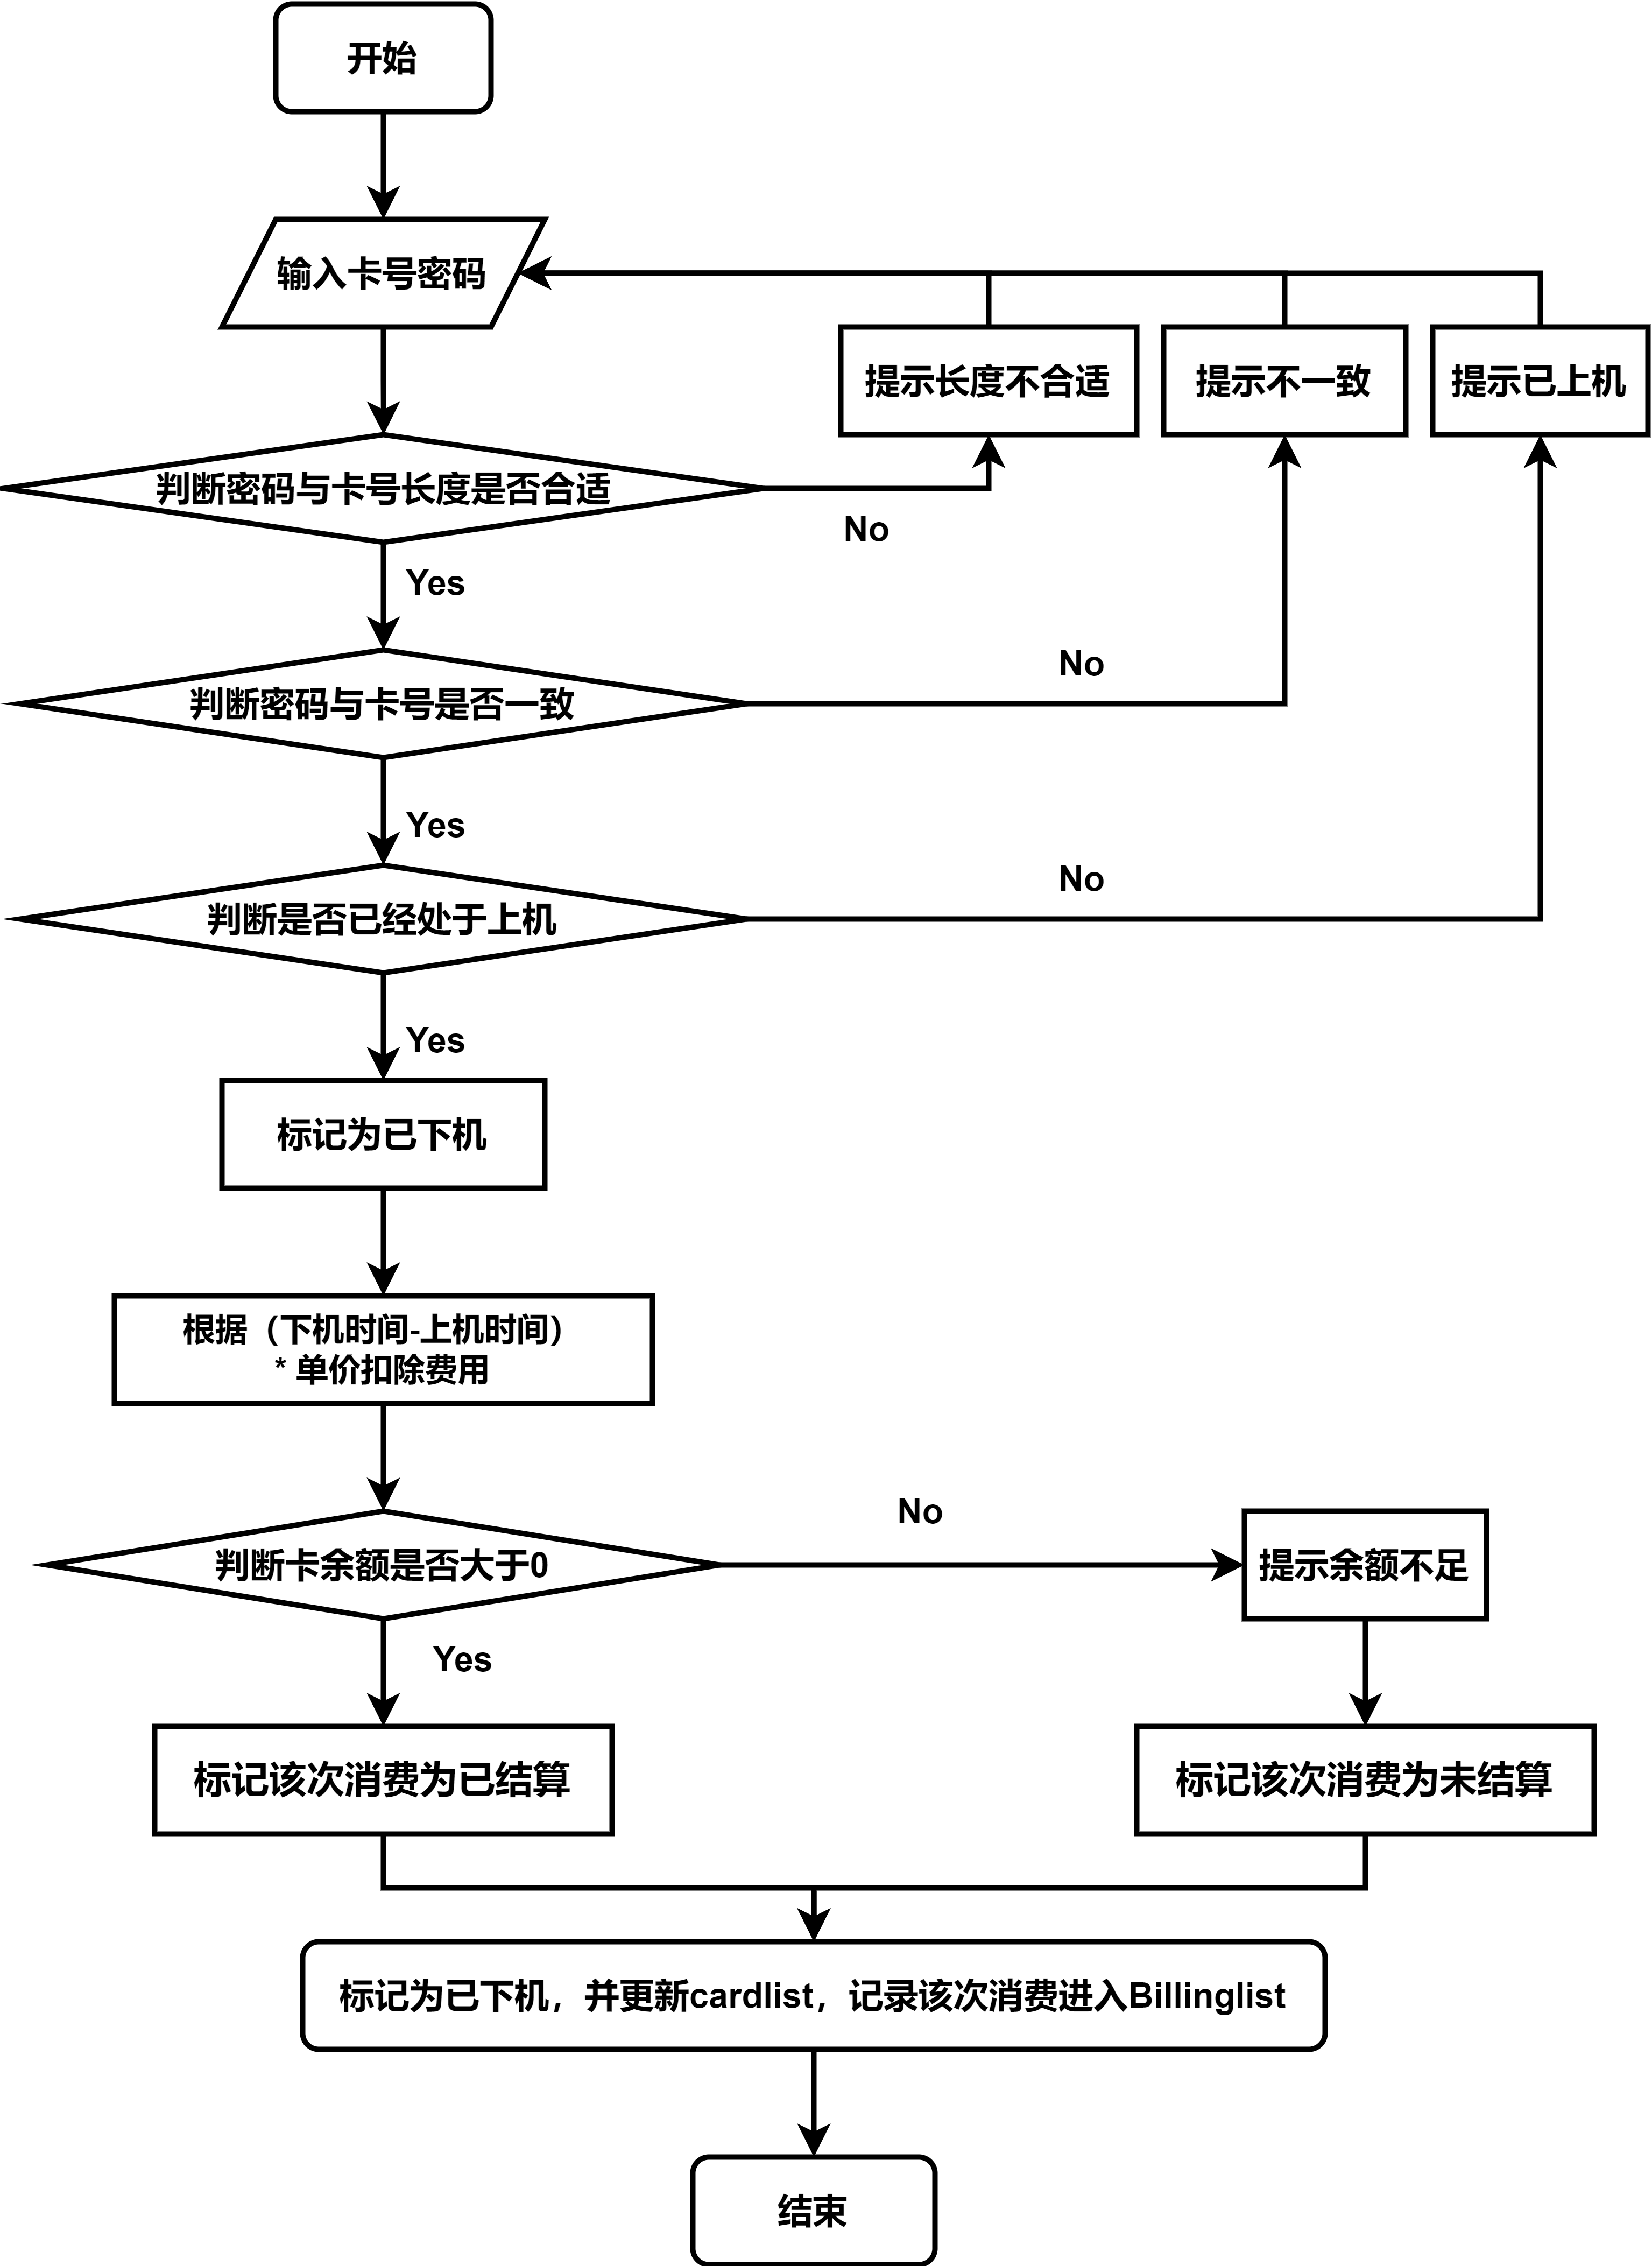
\includegraphics[scale=0.11]{figure/settle_pic.png}
        \caption{下机流程图}
        \label{settle_pic}
    \end{figure}
    如图\ref{settle_pic}为下机的流程图,首先判断是否存在输入长度过长问题,然后遍历链表cardlist判断是否该卡是否存在,该卡密码是否正确,
    再判断是否已经处于上机状态,通过后把该卡标记为下机,同时扣除费用(下机费用-上机费用)* 每秒金额,如果扣除后余额小于等于0,就提示余额不够,标记该次消费
    为未结算,并分别保存卡信息与消费到card.ams,billing.ams.
    \newpage
    \subsection{充值流程图}
    \begin{figure}[h]
        \centering
        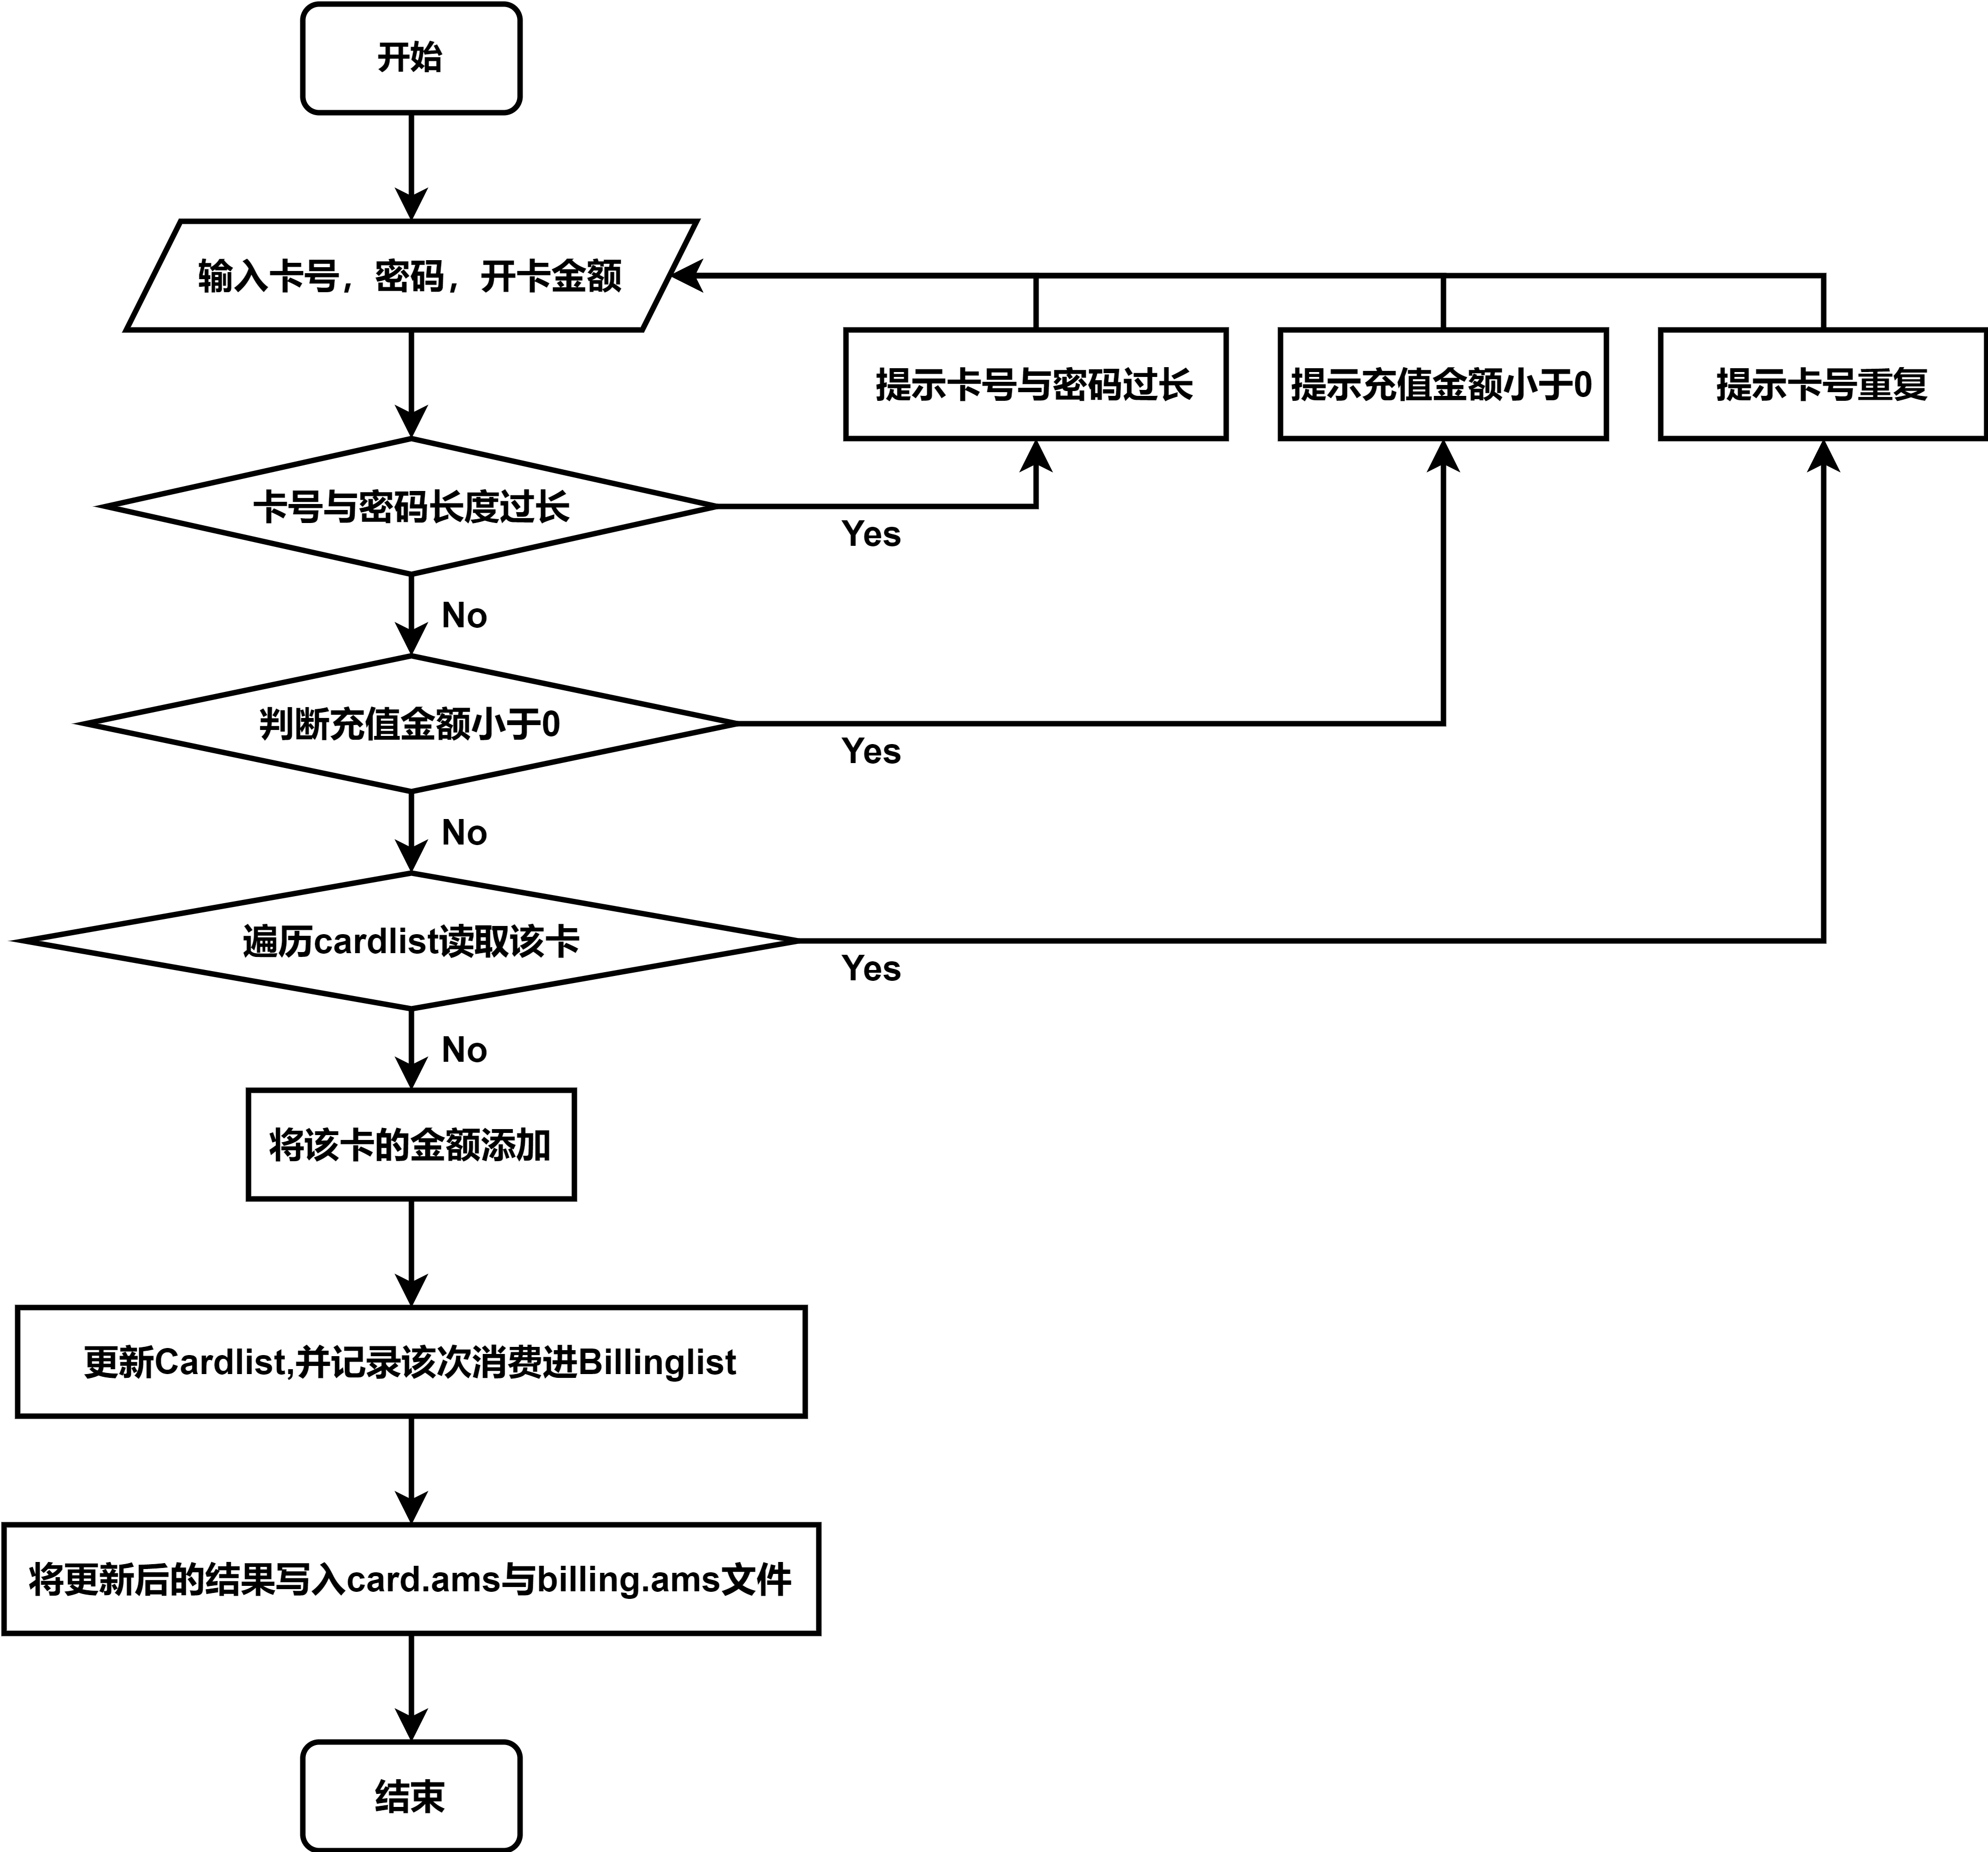
\includegraphics[scale=0.125]{figure/addmoney_pic.png}
        \caption{充值流程图}
        \label{addmoney_pic}
    \end{figure}
    如图\ref{addmoney_pic}为充值的流程图,首先判断是否存在输入非数字,长度过长问题,然后遍历链表cardlist判断是否该卡密码是否正确,
    再增加该卡金额,更新Cardlist,billing,将更新结果写入card.ams,billing.ams.
    \newpage
    \subsection{退款流程图}
    \begin{figure}[!h]
        \centering
        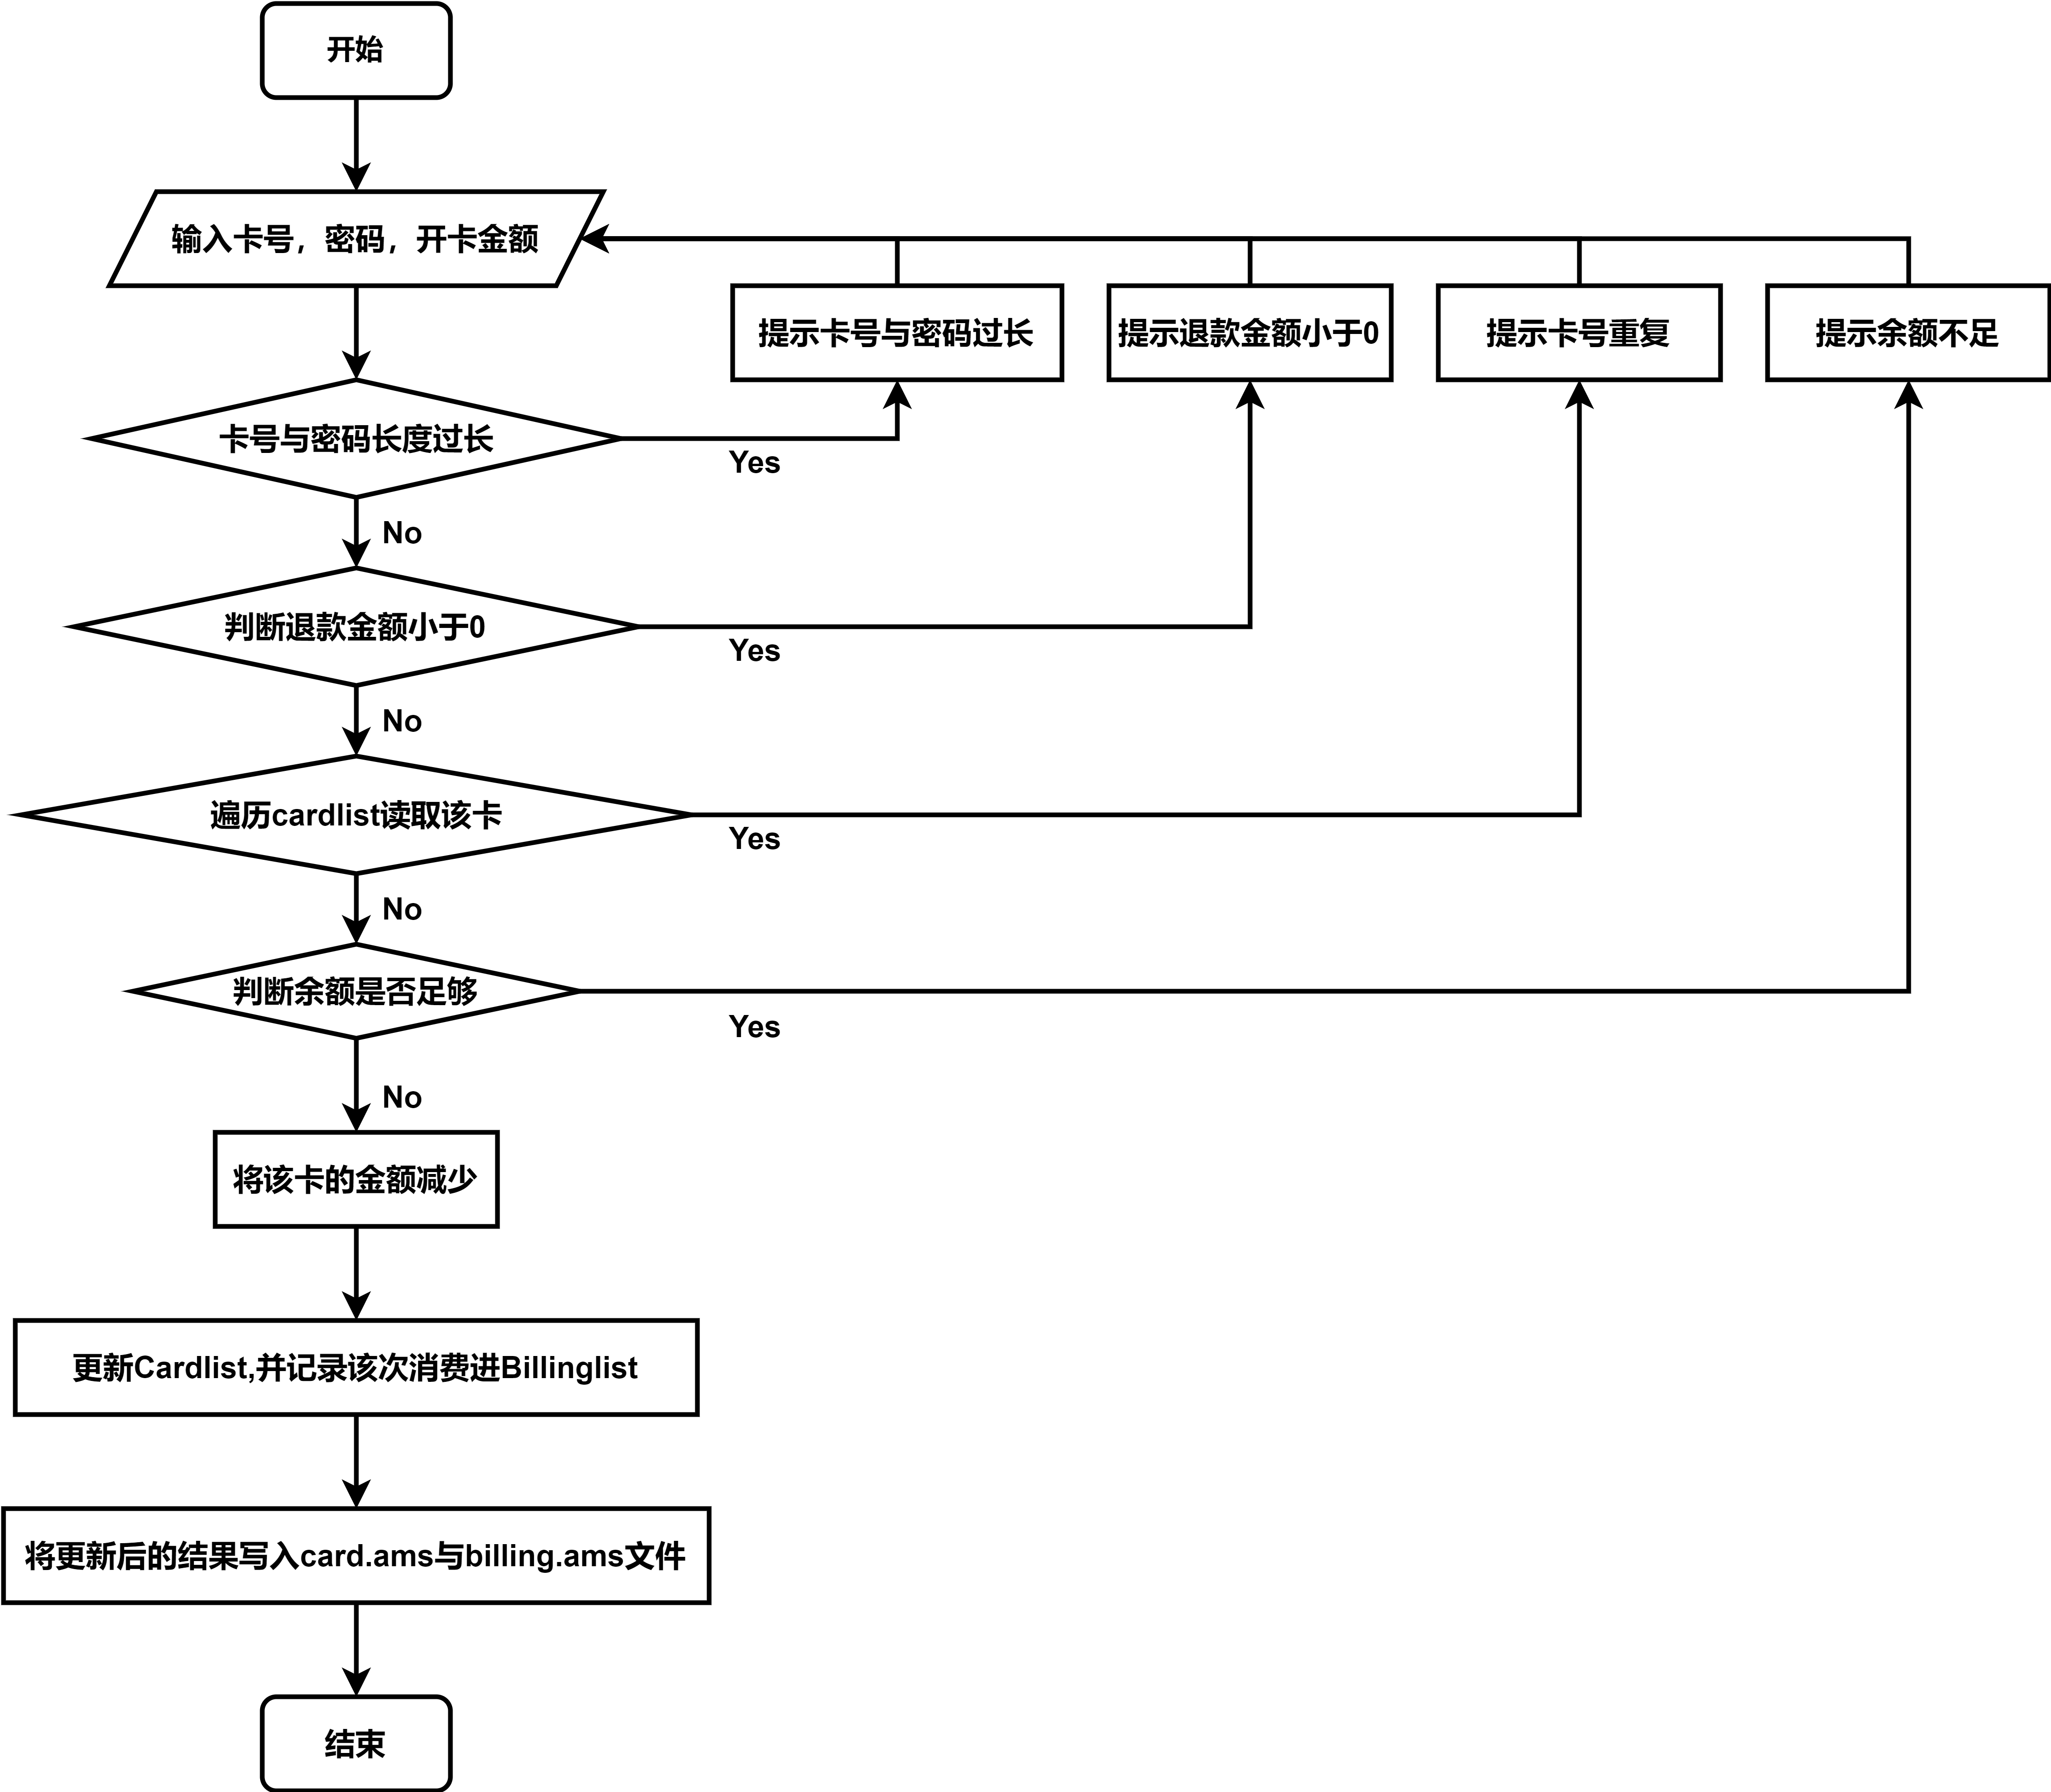
\includegraphics[scale=0.11]{figure/refund_pic.png}
        \caption{退款流程图}
        \label{refund_pic}
    \end{figure}
    如图\ref{refund_pic}为退款的流程图,首先判断是否存在输入非数字,长度过长问题,然后遍历链表cardlist判断是否该卡密码是否正确,
    再判断该卡是否余额足够,减少该卡金额,更新Cardlist,billing,将更新结果写入文件
    \newpage
    \subsection{注销流程图}
    \begin{figure}[!h]
        \centering
        \includegraphics[scale=0.125]{figure/annul_pic.png}
        \caption{注销流程图}
        \label{annul_pic}
    \end{figure}
    如图\ref{annul_pic}为注销的流程图,首先判断是否存在输入长度过长问题,然后遍历链表cardlist判断是否该卡是否存在,该卡密码是否正确,
    再判断是否已经处于下机状态,是否余额足够,通过后把删除该卡,并分别保存卡信息到card.ams.
    \newpage
    \section{开发难点与体会}
    \subsection{多文件编写}
    \subsubsection{难点}   
    虽然VS提供非常方便的功能,但是不利于我们学习C++/C的编译步骤 。使用VSCode分文件编写C++程序并不像VS那样容易,不能直接简单的编译多个C++文件。
    Makefile编写复杂,不好使用。
    \subsubsection{解决办法}
    刚开始使用Cmake工具,通过编写以下Cmakelist.txt编译管理
    \begin{minted}{cmake}
    cmake_minimum_required(VERSION 3.0)
    project(dev)
    set(EXECUTABLE_OUTPUT_PATH ${PROJECT_SOURCE_DIR}/bin)
    aux_source_directory(src SRC_LIST)
    set(SRC_LIST src/model/node/*.cpp 
                src/model/linklist/*.cpp
                src/view/*.cpp
                src/service/service.cpp
                src/main.cpp)
    include_directories(include)
    add_executable(main ${SRC_LIST})
    \end{minted}
    后来使用Qt后,通过Qmake编译管理多文件系统。
    \subsubsection{体会}
    \begin{itemize}
        \item 相比单文件,这次多文件需要更加良好的编译管理工具.
        \item  同时熟悉了C++/C的编译过程,如图\ref{cpp_complie}所示。
    \end{itemize}
    \begin{figure}[h]
        \centering
        \includegraphics[scale=0.08]{figure/cppcompile.png}
        \caption{编译过程}
        \label{cpp_complie}
    \end{figure}
    \subsection{较难理解链表}
    \subsubsection{难点}
    该次程序使用了链表作为存储数据结构,学习链表较难理解链表构建,编写链表容易出现野指针,空指针问题导致运行错误。
    \subsubsection{解决办法}
    \begin{figure}[h]
        \centering
        \includegraphics[scale=0.1]{figure/linklist_add.png}
        \caption{链表添加}
        \label{linklist_add}
    \end{figure}
    通过画一些简单的图进行辅助,看图编写程序。例如根据图\ref{linklist_add},编写以下链表添加代码。
    \begin{minted}{cpp}
        //第一步
        Billing* r = head;
        Billing* n = new Billing(billing), *temp = r->next;
        //第二步
        r->next = n;
        n->next = temp;
    \end{minted}
    \subsubsection{体会}
    \begin{itemize}
        \item 很多算法与数据结构知识点,单看文字表述概念可能比较枯燥,难以理解,所以有时我们可以通过边画图边编程来辅助我们理解每一步的过程
        \item 遇到一些运行错误可以使用printf,qDebug等函数进行锁定错误原因,从而改正错误。
        \item 遇到不懂的需要多看B站或者Mooc上的视频同时自己实操才能慢慢掌握。
    \end{itemize}
    \subsection{GUI编写}
    \subsubsection{难点}
    该次程序多次需要跳转页面,在这个过程容易出现野指针,数据无法同步等问题,自己写的页面并不美观,同时总是存在各种小bug.
    \subsubsection{解决办法}
    \begin{figure}[h]
        \centering
        \includegraphics[scale=0.1]{figure/qt_change.png}
        \caption{QT跳转页面}
        \label{QTchange}
    \end{figure}
    如图\ref{QTchange}。为页面跳转的方式,通过信号与槽来实现页面跳转,用connect绑定信号与槽实现页面跳转。
    每次退出后都及时退出该窗口,同时通过指针传递来实现不同页面信息的共享。对于页面不美观,我使用qss美化页面,
    同时自己绘制不少图片来形象展示功能。
    \subsubsection{体会}
    \begin{itemize}
        \item 信号与槽是QT强大的工具,可以轻松实现类信息的共享。
        \item 如果只是目前不展示该页面,则将页面隐藏,而不是销毁。
        \item 使用指针传递来实现跳转页面的信息共享。
        \item 圆角页面感觉相比直角看起来更舒服。
    \end{itemize}
    \newpage
    \section{实验总结}
        \subsection{收获与成长}
        \begin{enumerate}
            \item 多文件:这次实验我学习接触到多文件编写c/c++,以前都是单文件,而这次是多文件,刚开始多文件直接在vscode上面跑总是显示错误,后来
            通过上网找到需要用cmake做编译管理工具,所以我自己编写了CMakelist.txt,才能成功运行程序。
            \item 程序结构:这次程序功能较多。需要一个比较好的设计,根据网上查找资料与学校课程,我大致采用MVC架构,Model主要负责对于数据的处理,
            Service负责联系Model与View数据交互,View负责页面展示。这样设计可以方便实现从CLI程序到GUI程序过渡而不修改大量代码。
            \item 链表:这次实验使用了链表,虽然这是个简单的数据结构,但是刚开始学确实很吃力,概念不理解,指针容易到处“乱窜”。后来在b站与Mooc上看了
            不少视频才逐渐理解链表,后来编写时边画草图边写才写出来。
            \item GUI:该次程序也是我第一次写GUI程序,大一上写的基本都是CLI程序,输入输出处理简单,不需下太大功夫,而GUI程序需要简洁漂亮的画面来展示,
            需要设计页面的跳转,同时也需要对用户输入进行一定判断,防止意外导致程序崩溃,这也我感受到程序员应该“把简单留给用户,把复杂留给自己”。
        \end{enumerate}
        \subsection{反思与不足}
        \begin{enumerate}
            \item 代码可重复利用性并不高:我觉得QMenu,Qadd,Qaddmoney等类的作用相似,结构差不多,所以应该可以设计一个父类包括所有共性功能,再通过继承来减少代码重用,但是一直想不出一个合适的父类。
            而且linklist中的billinglist与cardlist结构也类似,都为链表,以后打算学习用泛型编程来做一个linklist模板类来减少重复写两次链表。
            \item GUI页面不优美:我大部分采用QT自带的控件,一般都不好看。以后还要继续学习QT,学习自定义定义控件,使画面更加多样好看,对用户友好。
            \item 部分数据不灵活:每秒的扣钱数,管理员的账户密码都是写死在global.h里,这些数据只能在源码里修改。以后打算通过json确定配置,这样更加灵活方便。
            \item 密码都是明文保存:容易泄露。明文密码容易导致个人信息的丢失,例如CSDN就出现明文密码泄露事件。所以密码需要使用一种加密算法进行加密。以后有机会接触一下加密算法。
            \item 有些功能算法可以优化:比如字符串比较可以使用KMP等更好的算法来提高速度等,随着程序增大,更优的算法可以提高运行速度。
        \end{enumerate}
        \subsection{感想}
        计算机世界的水很深,需要我们不断学习新知识,多实践,时刻保持谦虚好学态度,相信我们终将在信息海洋中乘风破浪。
    \includepdf[page=3]{figure/程序设计综合实验报告.pdf}
\end{document}